\documentclass[11pt]{article}

\usepackage[margin=1in]{geometry}
\usepackage{amsmath}
\usepackage{amssymb}
\usepackage{booktabs}
\usepackage{caption}
\usepackage{subcaption}
\usepackage{graphicx}
\usepackage{placeins}
\usepackage{float}
\usepackage[colorlinks=true,linkcolor=blue,urlcolor=blue,citecolor=blue]{hyperref}

\captionsetup{font=small,labelfont=bf}
\setlength{\parindent}{0pt}
\setlength{\parskip}{0.55em}

\title{Empirical Report: PTB Softmax-bigram model Experiments}
\author{}
\date{\today}

\begin{document}
\maketitle

\section{Experimental Setup}

\paragraph{Data.}
The dataset is the prepared Penn Treebank bigram file \texttt{ptb\_v5000.pt}, built from the PTB train split using whitespace tokenization and one appended \texttt{<eos>} token per line. The vocabulary size is fixed to \(V=5000\), with out-of-vocabulary words folded into \texttt{<unk>}. The train split contains 929,588 bigram observations and 206,760 nonzero bigram types, corresponding to a bigram density of 0.827\%. A descriptive analysis of the data distribution is provided in Section~\ref{sec:data-description}.

\paragraph{Model.}
For each context token \(x\) and target token \(y\), the model score is
\begin{equation}
z_{y|x}(W) = u_y^\top W e_x + b_y,
\end{equation}
where \(e_x \in \mathbb{R}^d\) and \(u_y \in \mathbb{R}^d\) are fixed random input and output representations, \(W \in \mathbb{R}^{d \times d}\) is the learned matrix, and \(b_y\) is a fixed output bias. The matrix \(W\) is initialized at zero in every trajectory. The experiment uses representation dimensions \(d \in \{128,256\}\) and representation seeds \(\{0,1,2\}\). For each seed, both \(E=[e_x]\) and \(U=[u_y]\) are sampled from a standard normal distribution and then column/row normalized to unit Euclidean norm.

\paragraph{Loss.}
Let \(\widehat p(x,y)\) denote the empirical train bigram distribution, \(\pi_x=\sum_y \widehat p(x,y)\) the empirical context marginal, and \(p_y=\sum_x \widehat p(x,y)\) the empirical target unigram marginal. The smoothed target distribution is
\begin{equation}
\widetilde p(x,y) = (1-\rho)\widehat p(x,y) + \rho\,\pi_x p_y,
\end{equation}
with \(\rho=10^{-3}\). The optimized training objective is the smoothed conditional cross-entropy
\begin{equation}
\mathcal{L}(W)
= \sum_x \pi_x \log\sum_y \exp(z_{y|x}(W))
- \sum_{x,y}\widetilde p(x,y)z_{y|x}(W).
\end{equation}
All curves in the results plot this training loss. The implementation evaluates the \(V \times V\) logits in chunks with at most 2,000,000 logit elements per chunk.

\paragraph{Bias initializations.}
Two fixed output-bias choices are evaluated. In the \texttt{unigram\_log} condition, \(b_y=\log p_y\), so the zero-\(W\) model starts from the empirical unigram target distribution. In the \texttt{zero} condition, \(b_y=0\), so the zero-\(W\) model starts from a uniform output distribution. Both conditions are run for \(d=128\) and \(d=256\), giving four main settings.

\paragraph{Optimization directions.}
Every optimizer forms an update direction from the full training gradient \(G_t=\nabla\mathcal{L}(W_t)\) and then applies \(W_{t+1}=W_t+\eta_t D_t\). The three constant-learning-rate directions are
\begin{align}
\text{GD:}\quad &D_t=-G_t,\\
\text{NGD:}\quad &D_t=-G_t/\lVert G_t\rVert_F,\\
\text{Muon:}\quad &D_t=-\mathrm{polar}(G_t),
\end{align}
where \(\mathrm{polar}(G_t)\) is the partial polar factor computed from the SVD with relative tolerance \(10^{-7}\). NGD therefore changes only the step-length parameterization relative to GD, while Muon changes the matrix direction by replacing singular values with ones on the retained singular subspace.

\paragraph{Constant-learning-rate sweeps.}
The constant-schedule block sweeps a fixed \(\eta\) for GD, NGD, and Muon. GD uses 29 log-spaced values from \(10^{-1}\) to \(10^6\), NGD uses 25 log-spaced values from \(10^{-3}\) to \(10^3\), and Muon uses 21 log-spaced values from \(10^{-4}\) to \(10^1\). The \texttt{unigram\_log} runs are evaluated for 150 steps, while the \texttt{zero} runs are evaluated for 200 steps. Each trajectory is run for all three representation seeds. High-\(\eta\) tail pruning is enabled after at least 8 completed \(\eta\) values and triggers after 3 consecutive unstable high-\(\eta\) runs beyond the best value seen so far.

\paragraph{Exact line search.}
The line-search block evaluates exact one-dimensional line search for GD and Muon directions. NGD exact line search is omitted because NGD and GD point along the same ray; exact search along \(-G_t/\lVert G_t\rVert_F\) would be equivalent to exact search along \(-G_t\) after rescaling \(\eta\). For GD line search, the initial bracket high value is 256 and the maximum allowed \(\eta\) is \(10^6\). For Muon line search, the initial bracket high value is 0.25 and the maximum allowed \(\eta\) is 20. The bracket grows by a factor of 2 for up to 16 bracket iterations, followed by 8 bisection iterations. The selected \(\eta_t\) is recorded at every update step.

\paragraph{Selection and aggregation.}
The full run contains 785 trajectories and 127,163 trace rows. Best constant learning rates are selected separately for each \((V,d,\rho,\text{bias},\text{optimizer})\) group using an AUC-style log-loss score,
\begin{equation}
s = \frac{1}{T+1}\sum_{t=0}^{T}\log\left(\max(\mathcal{L}(W_t),10^{-30})\right),
\end{equation}
averaged over the three representation seeds; lower is better. Unstable or missing seed trajectories are penalized during selection. The main comparison figures show the AUC-selected constant GD, NGD, and Muon curves together with exact line-search GD and Muon curves. All plotted curves are seed means, and shaded bands show one standard deviation across seeds.

\section{Results: Best Constants Versus Exact Line Search}

This section includes all figures from \texttt{main\_comparison} and \texttt{selected\_eta}. For each setting, the comparison figure is placed first and the selected line-search learning-rate schedule is placed second.

\begin{figure}[H]
\centering
\begin{subfigure}[t]{0.68\linewidth}
\centering
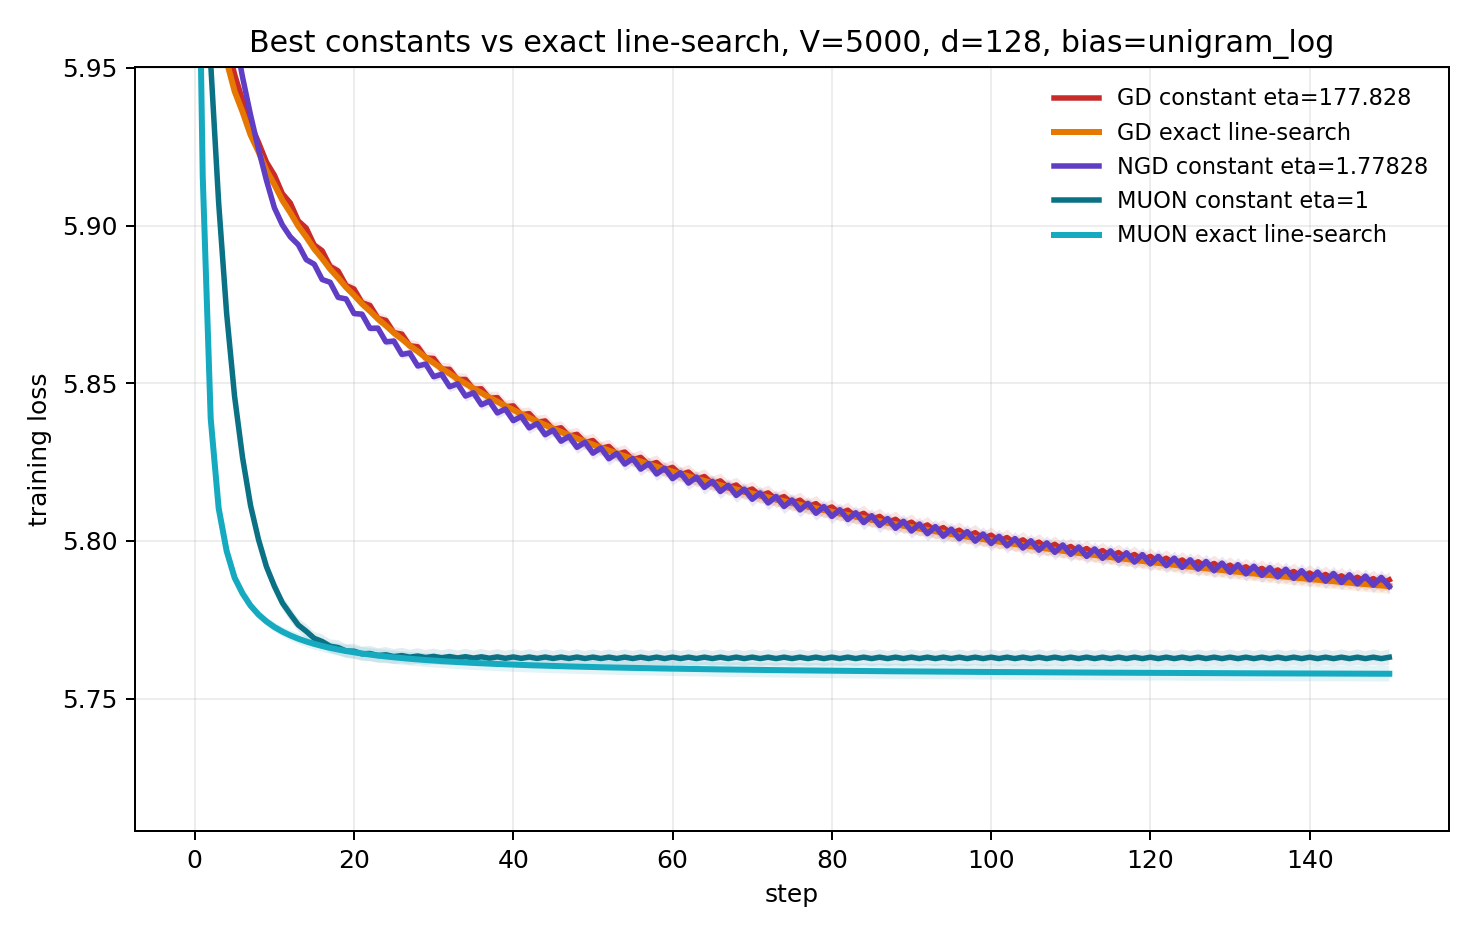
\includegraphics[width=\linewidth]{figures/report_figures/best_constant_vs_line_search_V5000_d128_rho1e-03_unigram_log.png}
\caption{Best constants versus exact line search.}
\end{subfigure}\hfill
\begin{subfigure}[t]{0.3\linewidth}
\centering
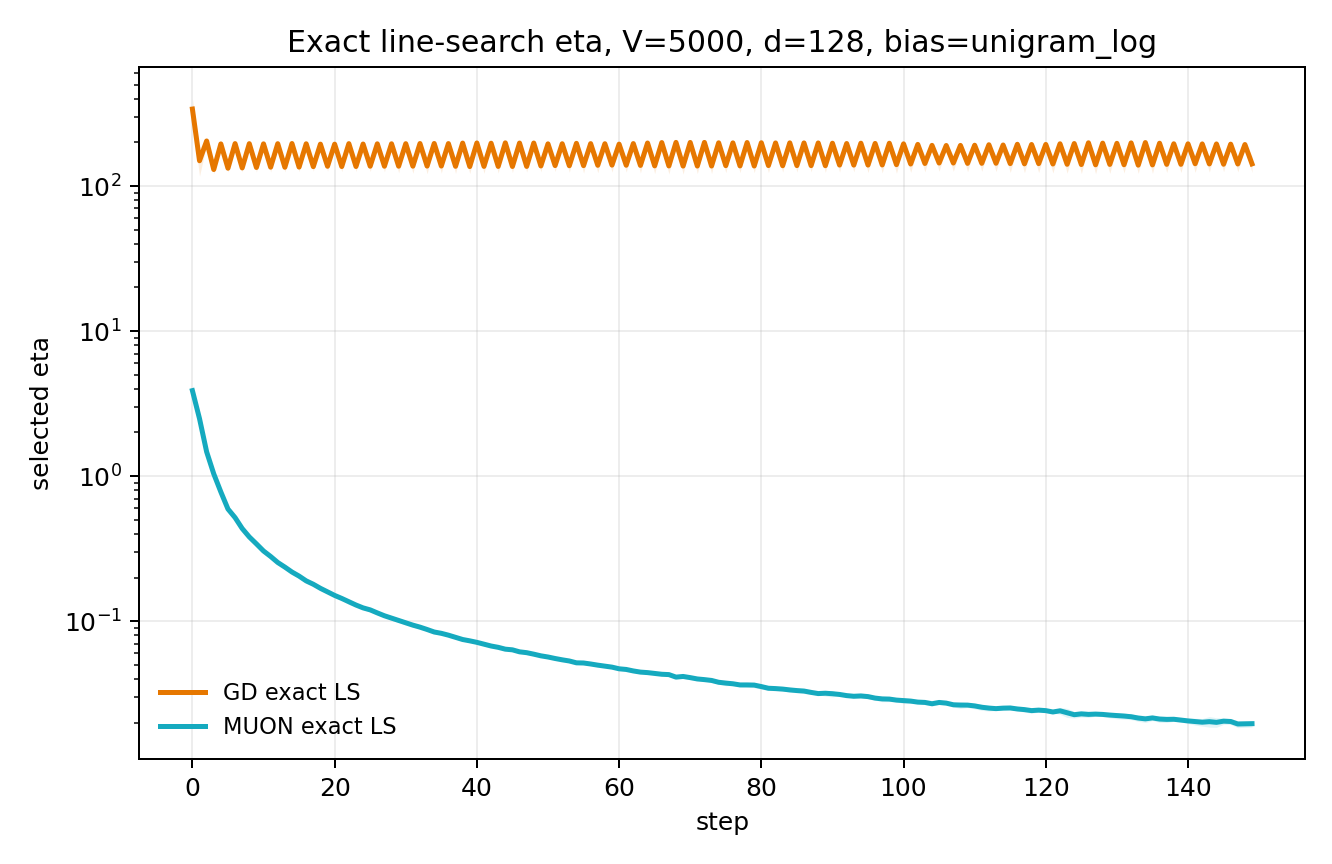
\includegraphics[width=\linewidth]{figures/report_figures/selected_eta_V5000_d128_rho1e-03_unigram_log.png}
\caption{Selected line-search learning rates.}
\end{subfigure}
\caption{\textbf{\(V=5000\), \(d=128\), \(\rho=10^{-3}\), \texttt{unigram\_log} bias.}
Left: training-loss comparison between AUC-selected constant GD, NGD, Muon and exact line-search GD/Muon. Right: selected \(\eta_t\) schedules for the exact line-search GD and Muon runs. Curves are seed means with one-standard-deviation bands.}
\label{fig:main-unigram-d128}
\end{figure}

\begin{figure}[H]
\centering
\begin{subfigure}[t]{0.68\linewidth}
\centering
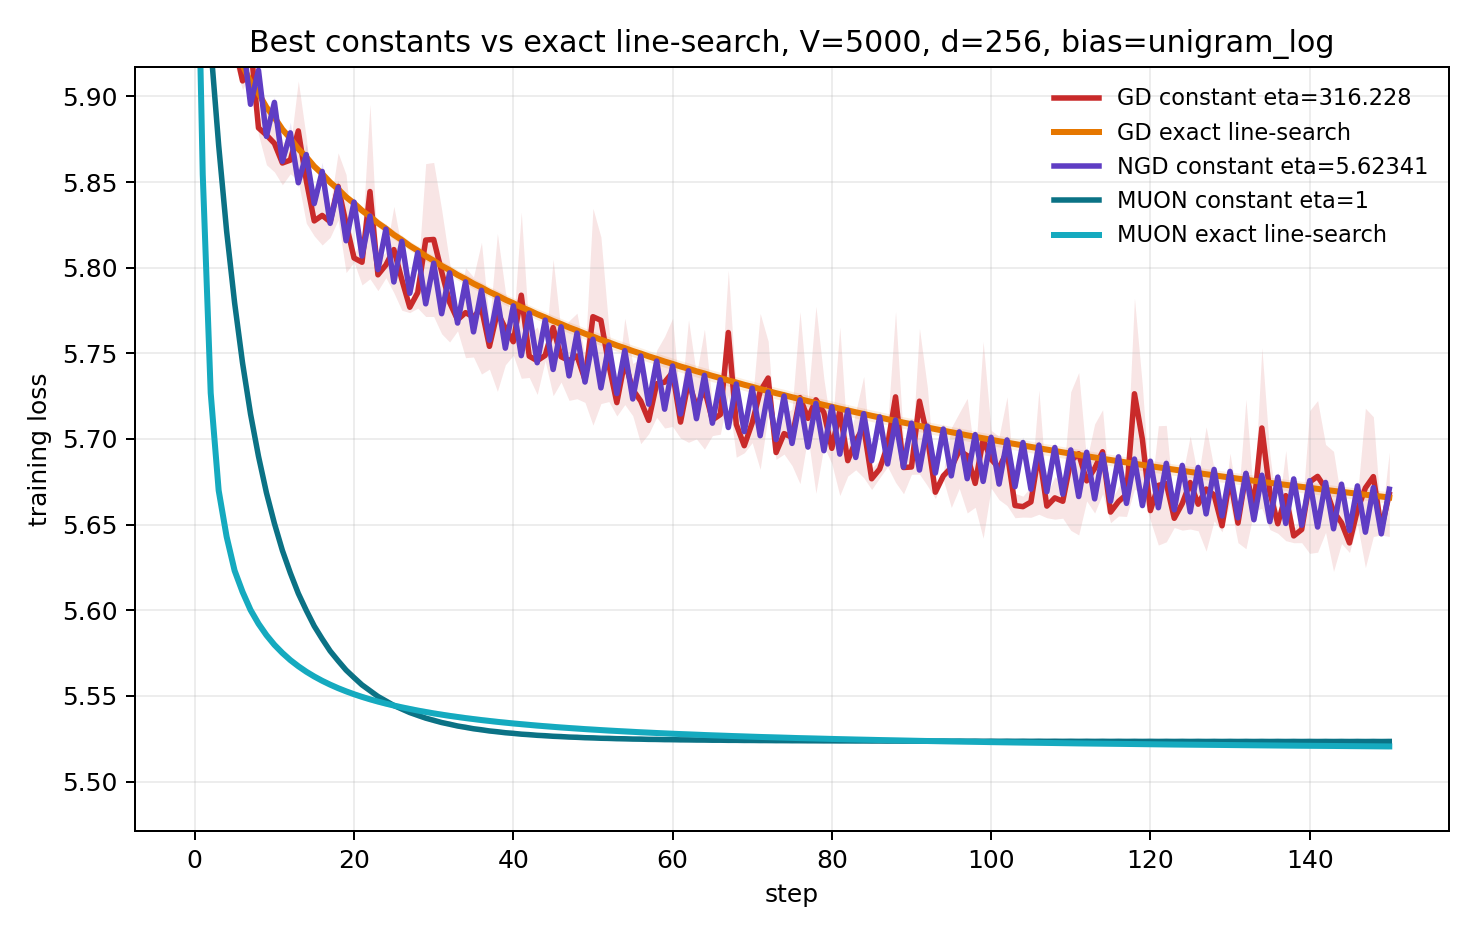
\includegraphics[width=\linewidth]{figures/report_figures/best_constant_vs_line_search_V5000_d256_rho1e-03_unigram_log.png}
\caption{Best constants versus exact line search.}
\end{subfigure}\hfill
\begin{subfigure}[t]{0.3\linewidth}
\centering
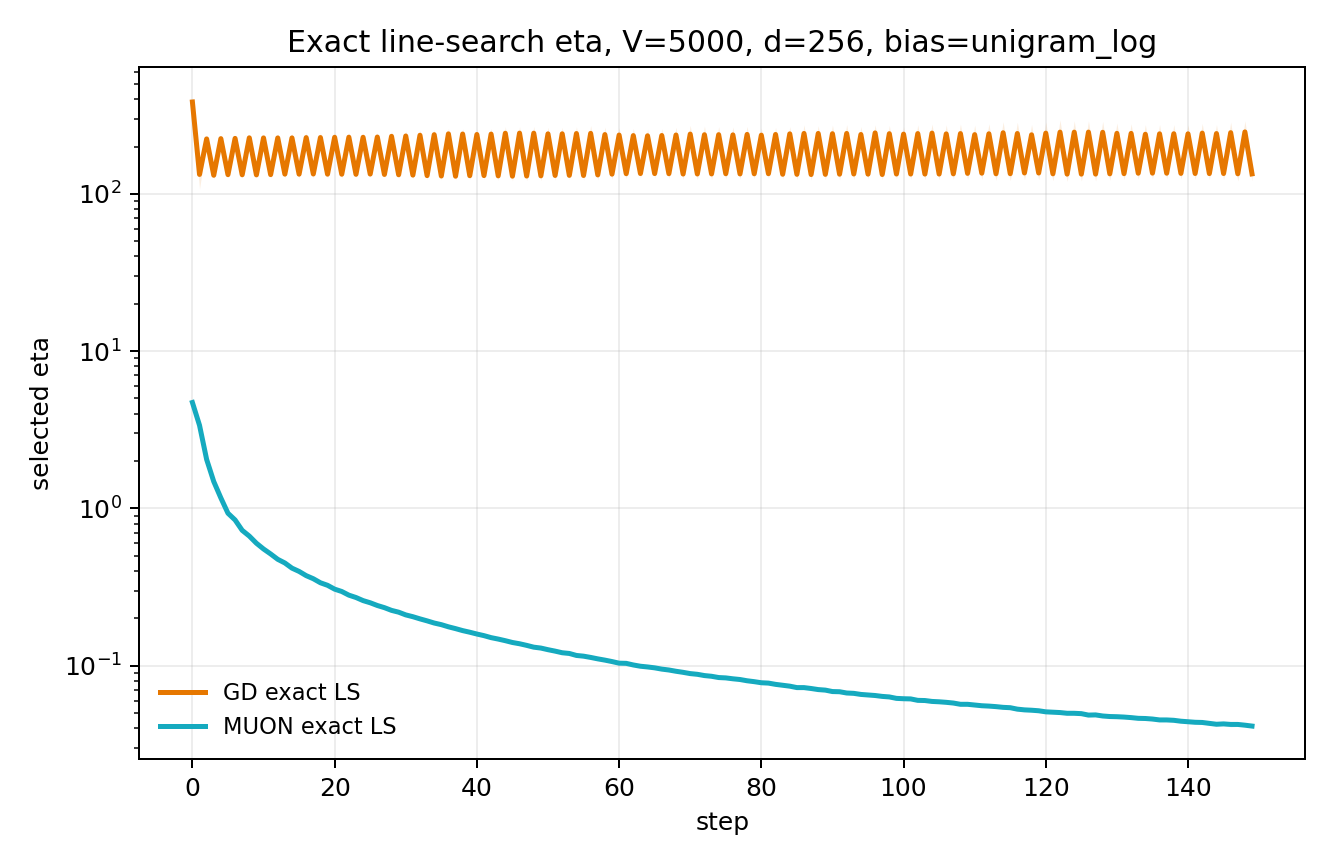
\includegraphics[width=\linewidth]{figures/report_figures/selected_eta_V5000_d256_rho1e-03_unigram_log.png}
\caption{Selected line-search learning rates.}
\end{subfigure}
\caption{\textbf{\(V=5000\), \(d=256\), \(\rho=10^{-3}\), \texttt{unigram\_log} bias.}
Left: training-loss comparison between AUC-selected constant GD, NGD, Muon and exact line-search GD/Muon. Right: selected \(\eta_t\) schedules for the exact line-search GD and Muon runs. Curves are seed means with one-standard-deviation bands.}
\label{fig:main-unigram-d256}
\end{figure}

\begin{figure}[H]
\centering
\begin{subfigure}[t]{0.68\linewidth}
\centering
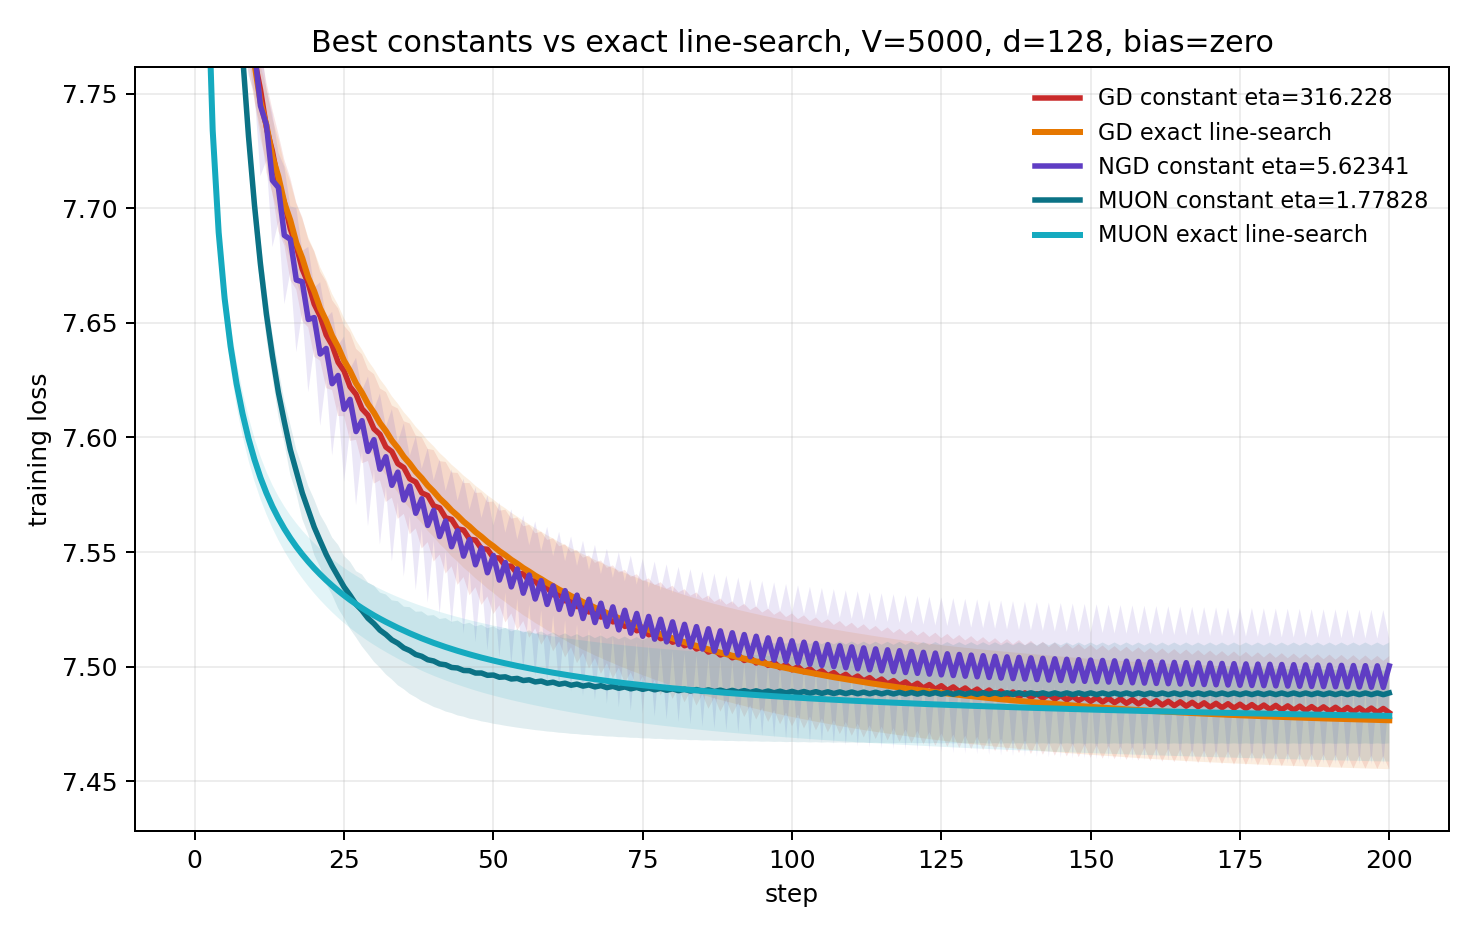
\includegraphics[width=\linewidth]{figures/report_figures/best_constant_vs_line_search_V5000_d128_rho1e-03_zero.png}
\caption{Best constants versus exact line search.}
\end{subfigure}\hfill
\begin{subfigure}[t]{0.3\linewidth}
\centering
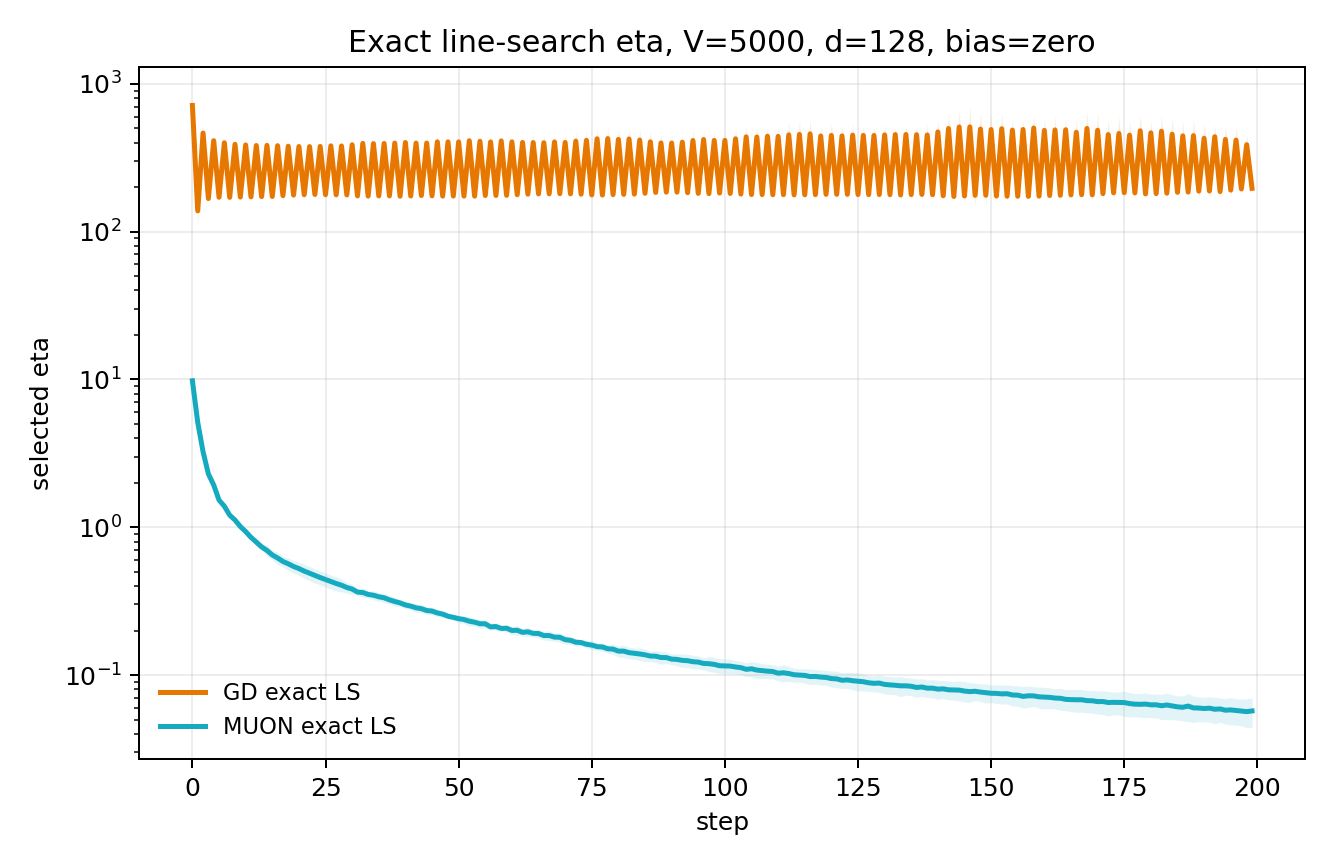
\includegraphics[width=\linewidth]{figures/report_figures/selected_eta_V5000_d128_rho1e-03_zero.png}
\caption{Selected line-search learning rates.}
\end{subfigure}
\caption{\textbf{\(V=5000\), \(d=128\), \(\rho=10^{-3}\), zero bias.}
Left: training-loss comparison between AUC-selected constant GD, NGD, Muon and exact line-search GD/Muon. Right: selected \(\eta_t\) schedules for the exact line-search GD and Muon runs. Curves are seed means with one-standard-deviation bands.}
\label{fig:main-zero-d128}
\end{figure}

\begin{figure}[H]
\centering
\begin{subfigure}[t]{0.68\linewidth}
\centering
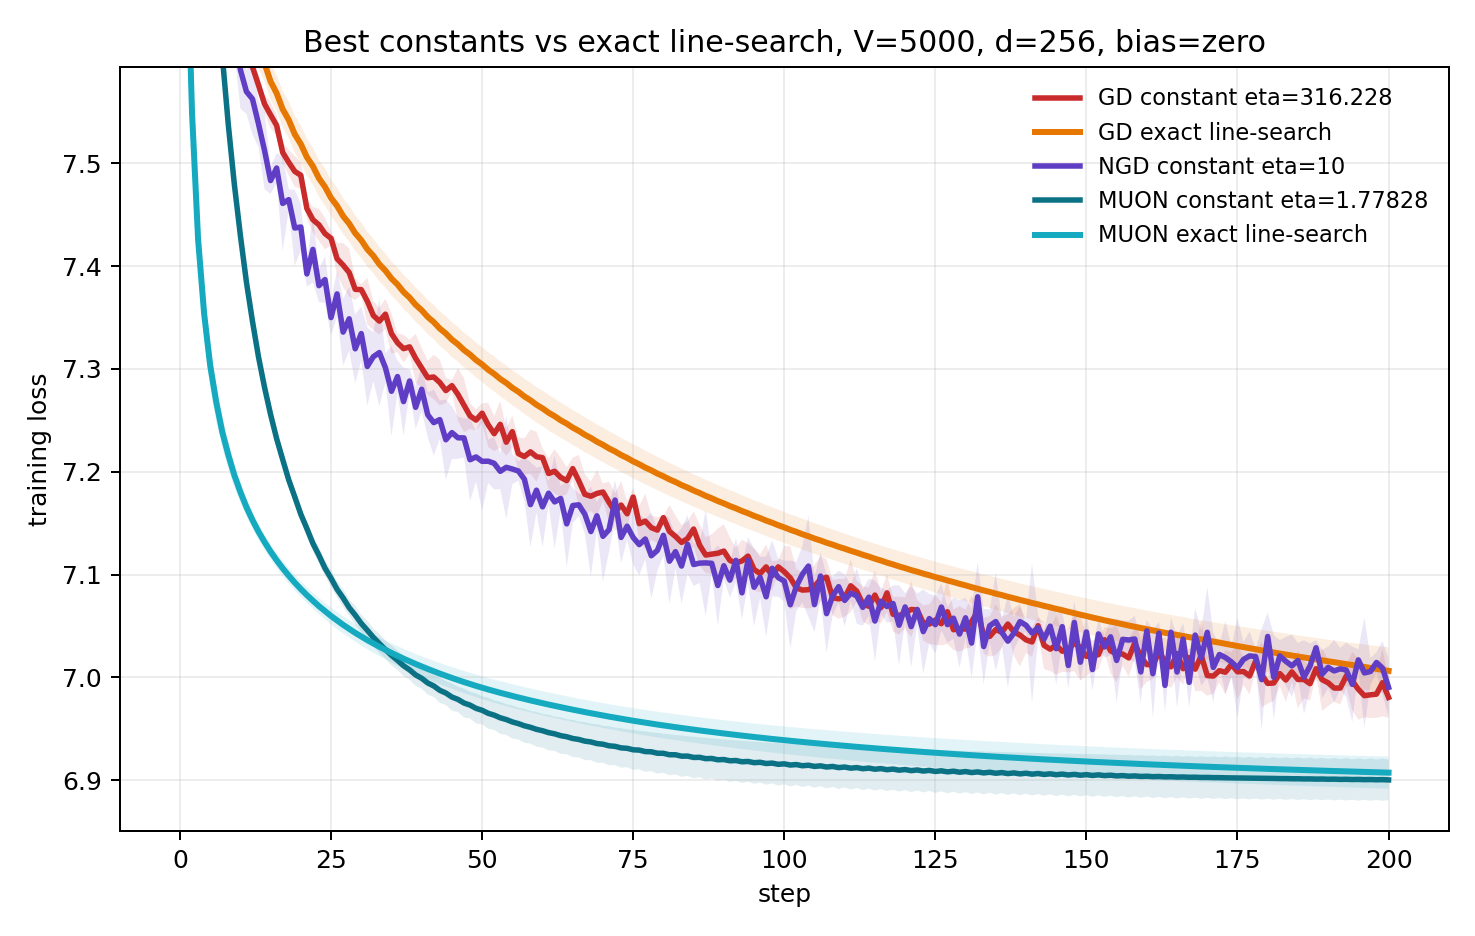
\includegraphics[width=\linewidth]{figures/report_figures/best_constant_vs_line_search_V5000_d256_rho1e-03_zero.png}
\caption{Best constants versus exact line search.}
\end{subfigure}\hfill
\begin{subfigure}[t]{0.3\linewidth}
\centering
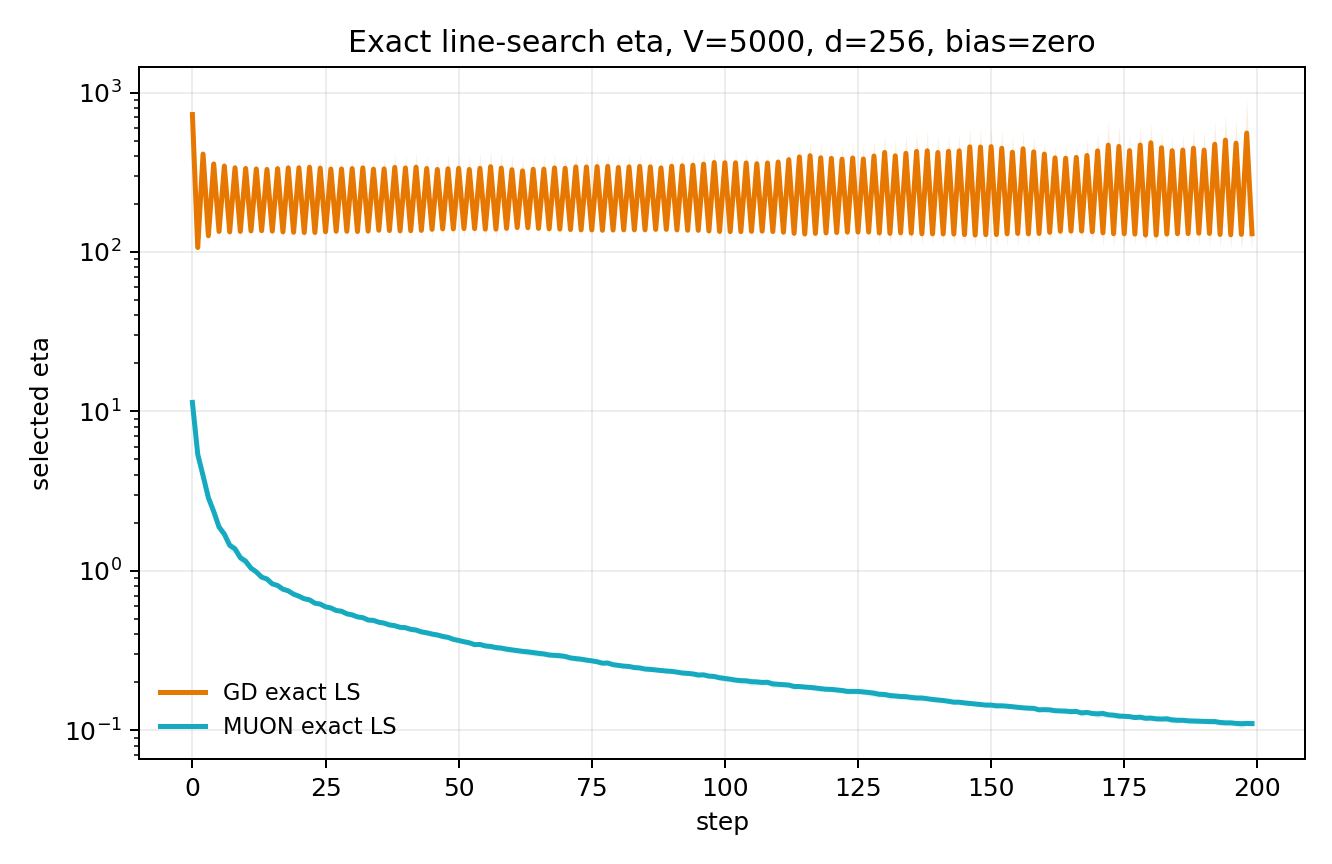
\includegraphics[width=\linewidth]{figures/report_figures/selected_eta_V5000_d256_rho1e-03_zero.png}
\caption{Selected line-search learning rates.}
\end{subfigure}
\caption{\textbf{\(V=5000\), \(d=256\), \(\rho=10^{-3}\), zero bias.}
Left: training-loss comparison between AUC-selected constant GD, NGD, Muon and exact line-search GD/Muon. Right: selected \(\eta_t\) schedules for the exact line-search GD and Muon runs. Curves are seed means with one-standard-deviation bands.}
\label{fig:main-zero-d256}
\end{figure}

\FloatBarrier
\section{Results: Constant Learning-Rate Sweeps}

This section includes the GD and NGD constant-sweep loss curves used for schedule selection. The Muon sweep figures themselves are intentionally omitted, but the GD/NGD sweep panels retain the AUC-selected Muon constant curve as a black reference baseline.

\begin{figure}[H]
\centering
\begin{subfigure}[t]{0.9\linewidth}
\centering
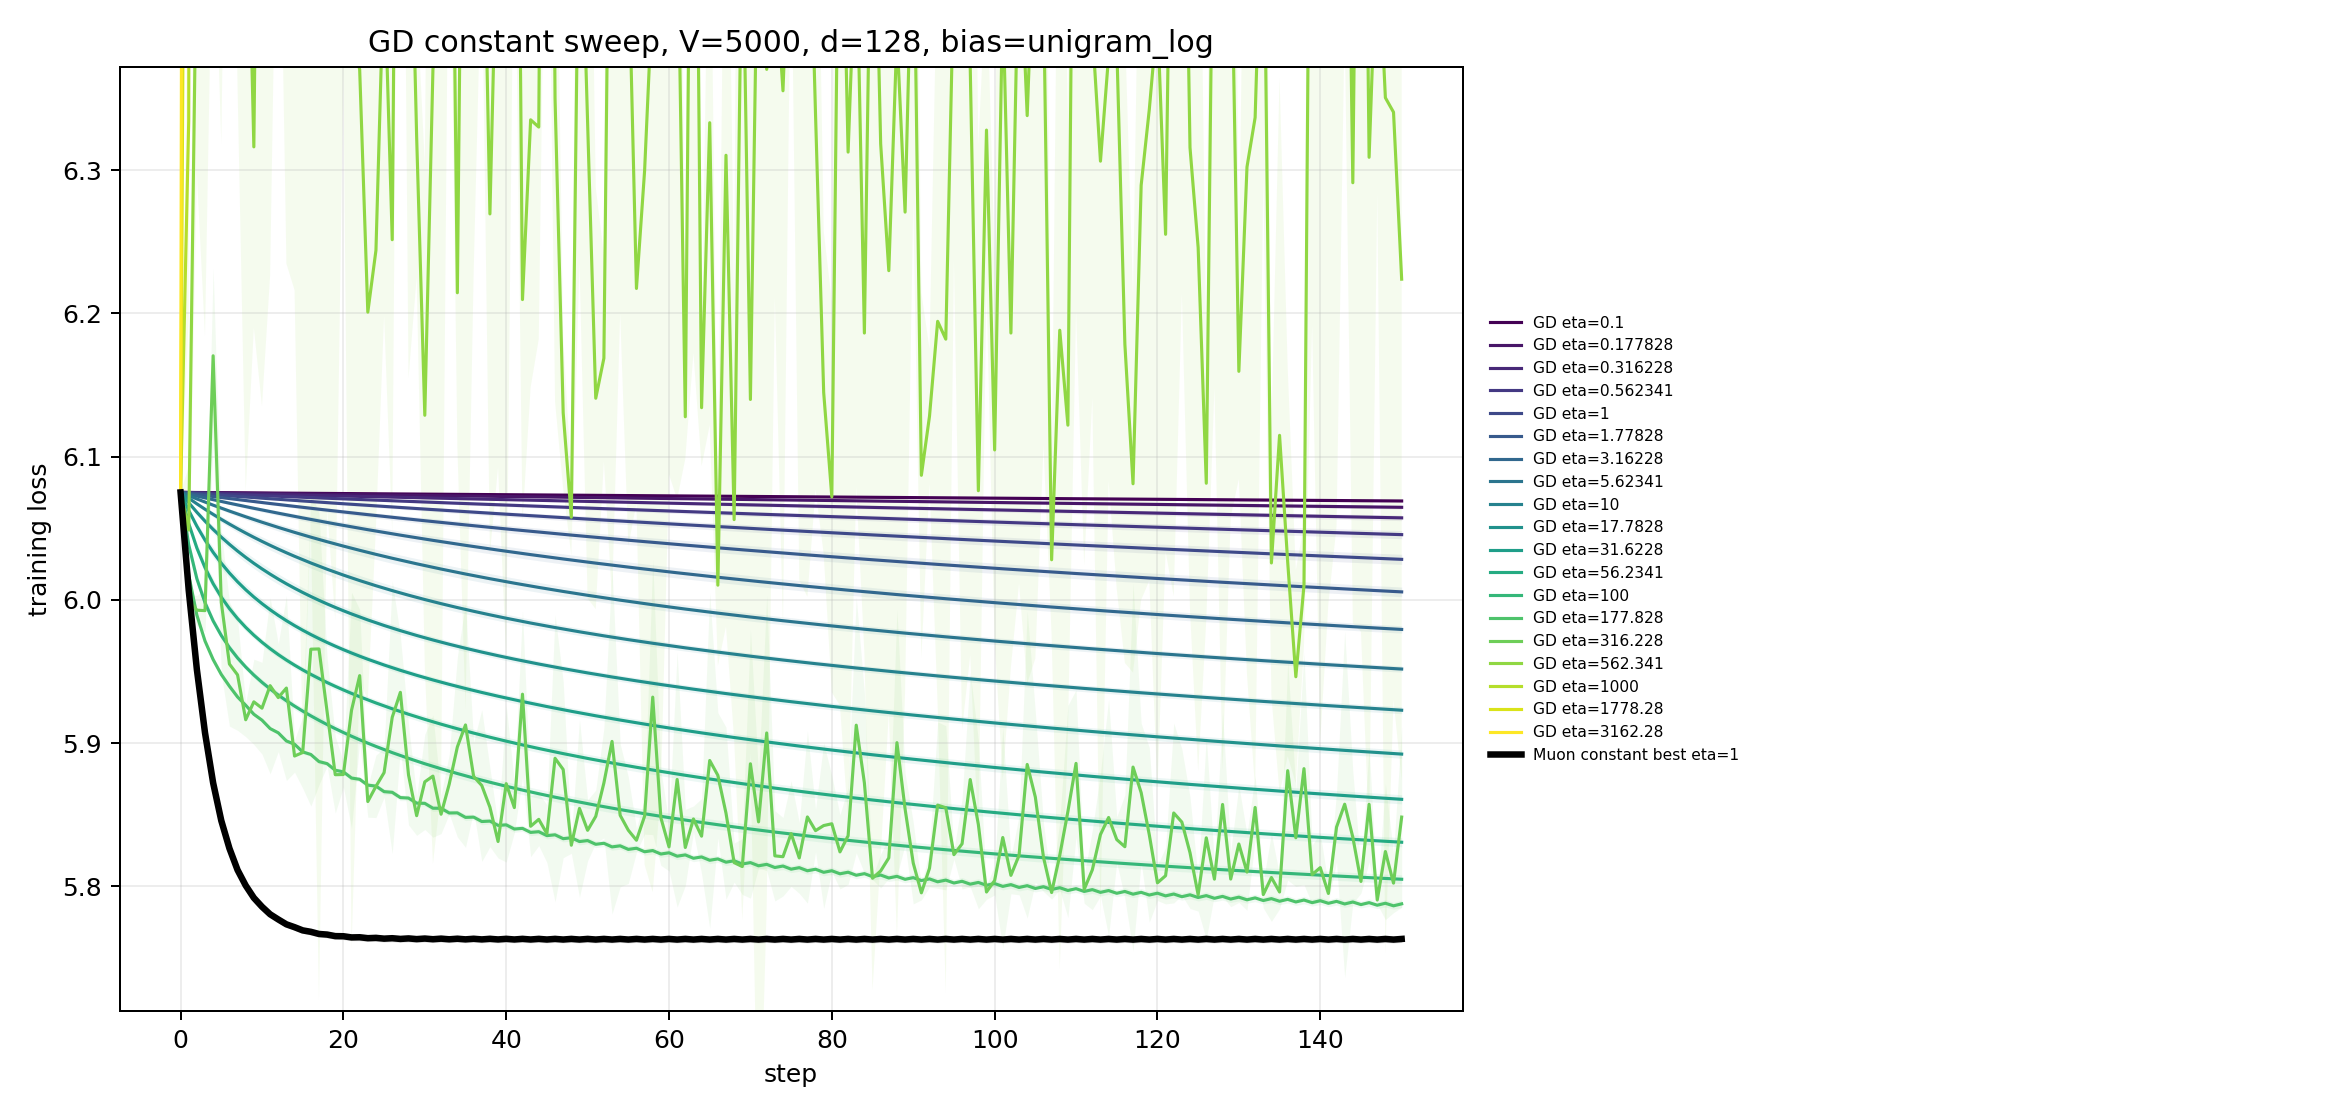
\includegraphics[width=\linewidth]{figures/report_figures/gd_constant_sweep_V5000_d128_rho1e-03_unigram_log.png}
\caption{GD sweep.}
\end{subfigure}\hfill
\begin{subfigure}[t]{0.9\linewidth}
\centering
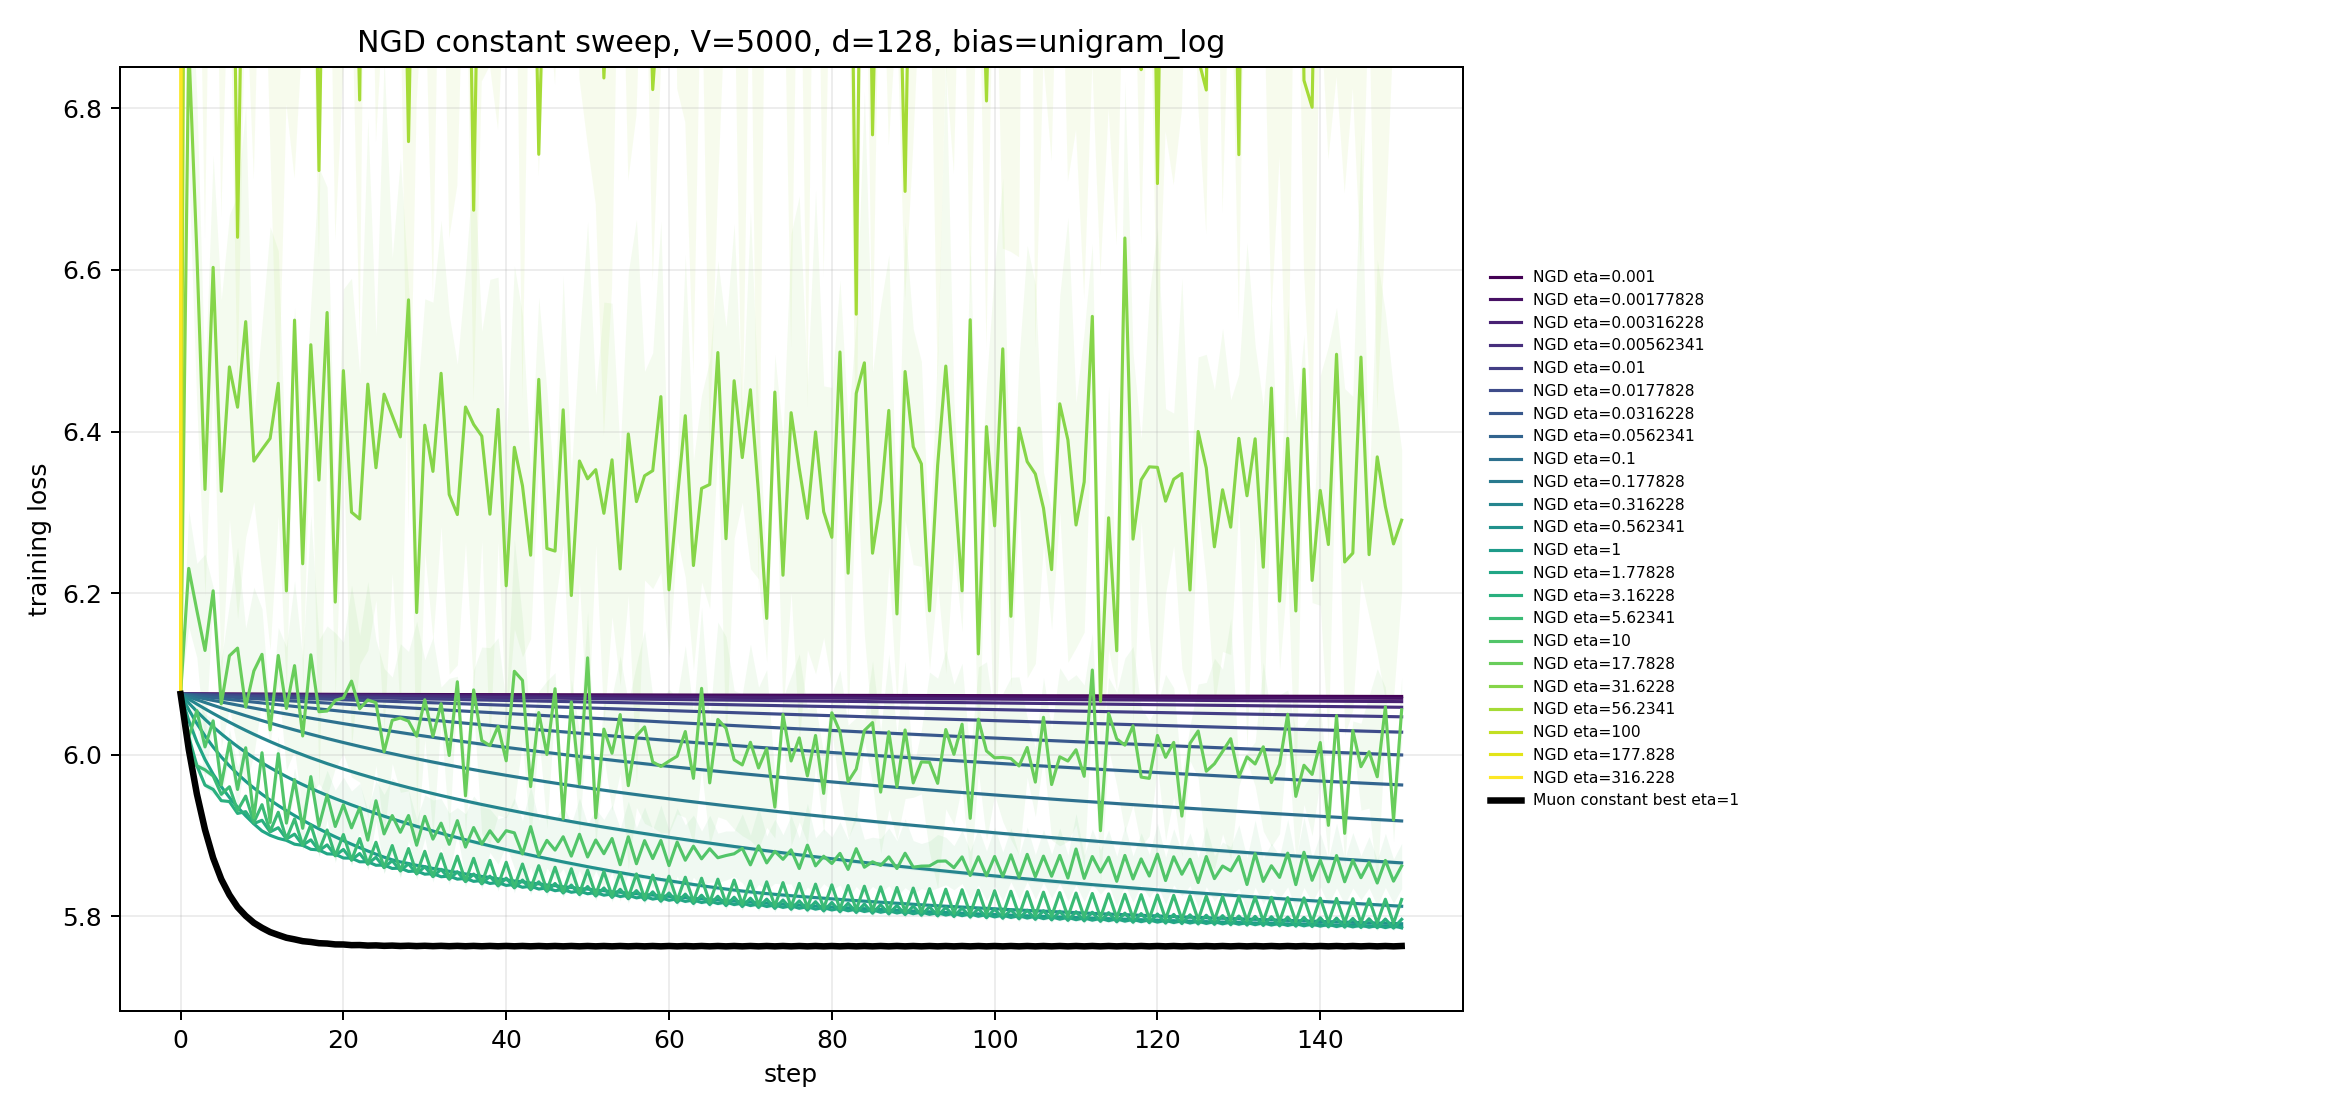
\includegraphics[width=\linewidth]{figures/report_figures/ngd_constant_sweep_V5000_d128_rho1e-03_unigram_log.png}
\caption{NGD sweep.}
\end{subfigure}
\caption{\textbf{\(V=5000\), \(d=128\), \(\rho=10^{-3}\), \texttt{unigram\_log} bias.}
Left: GD constant-\(\eta\) sweep loss curves. Right: NGD constant-\(\eta\) sweep loss curves. Each colored curve is one fixed GD/NGD \(\eta\); the black curve is the AUC-selected Muon constant baseline. Curves are seed means with one-standard-deviation bands.}
\label{fig:sweep-unigram-d128}
\end{figure}

\begin{figure}[H]
\centering
\begin{subfigure}[t]{0.9\linewidth}
\centering
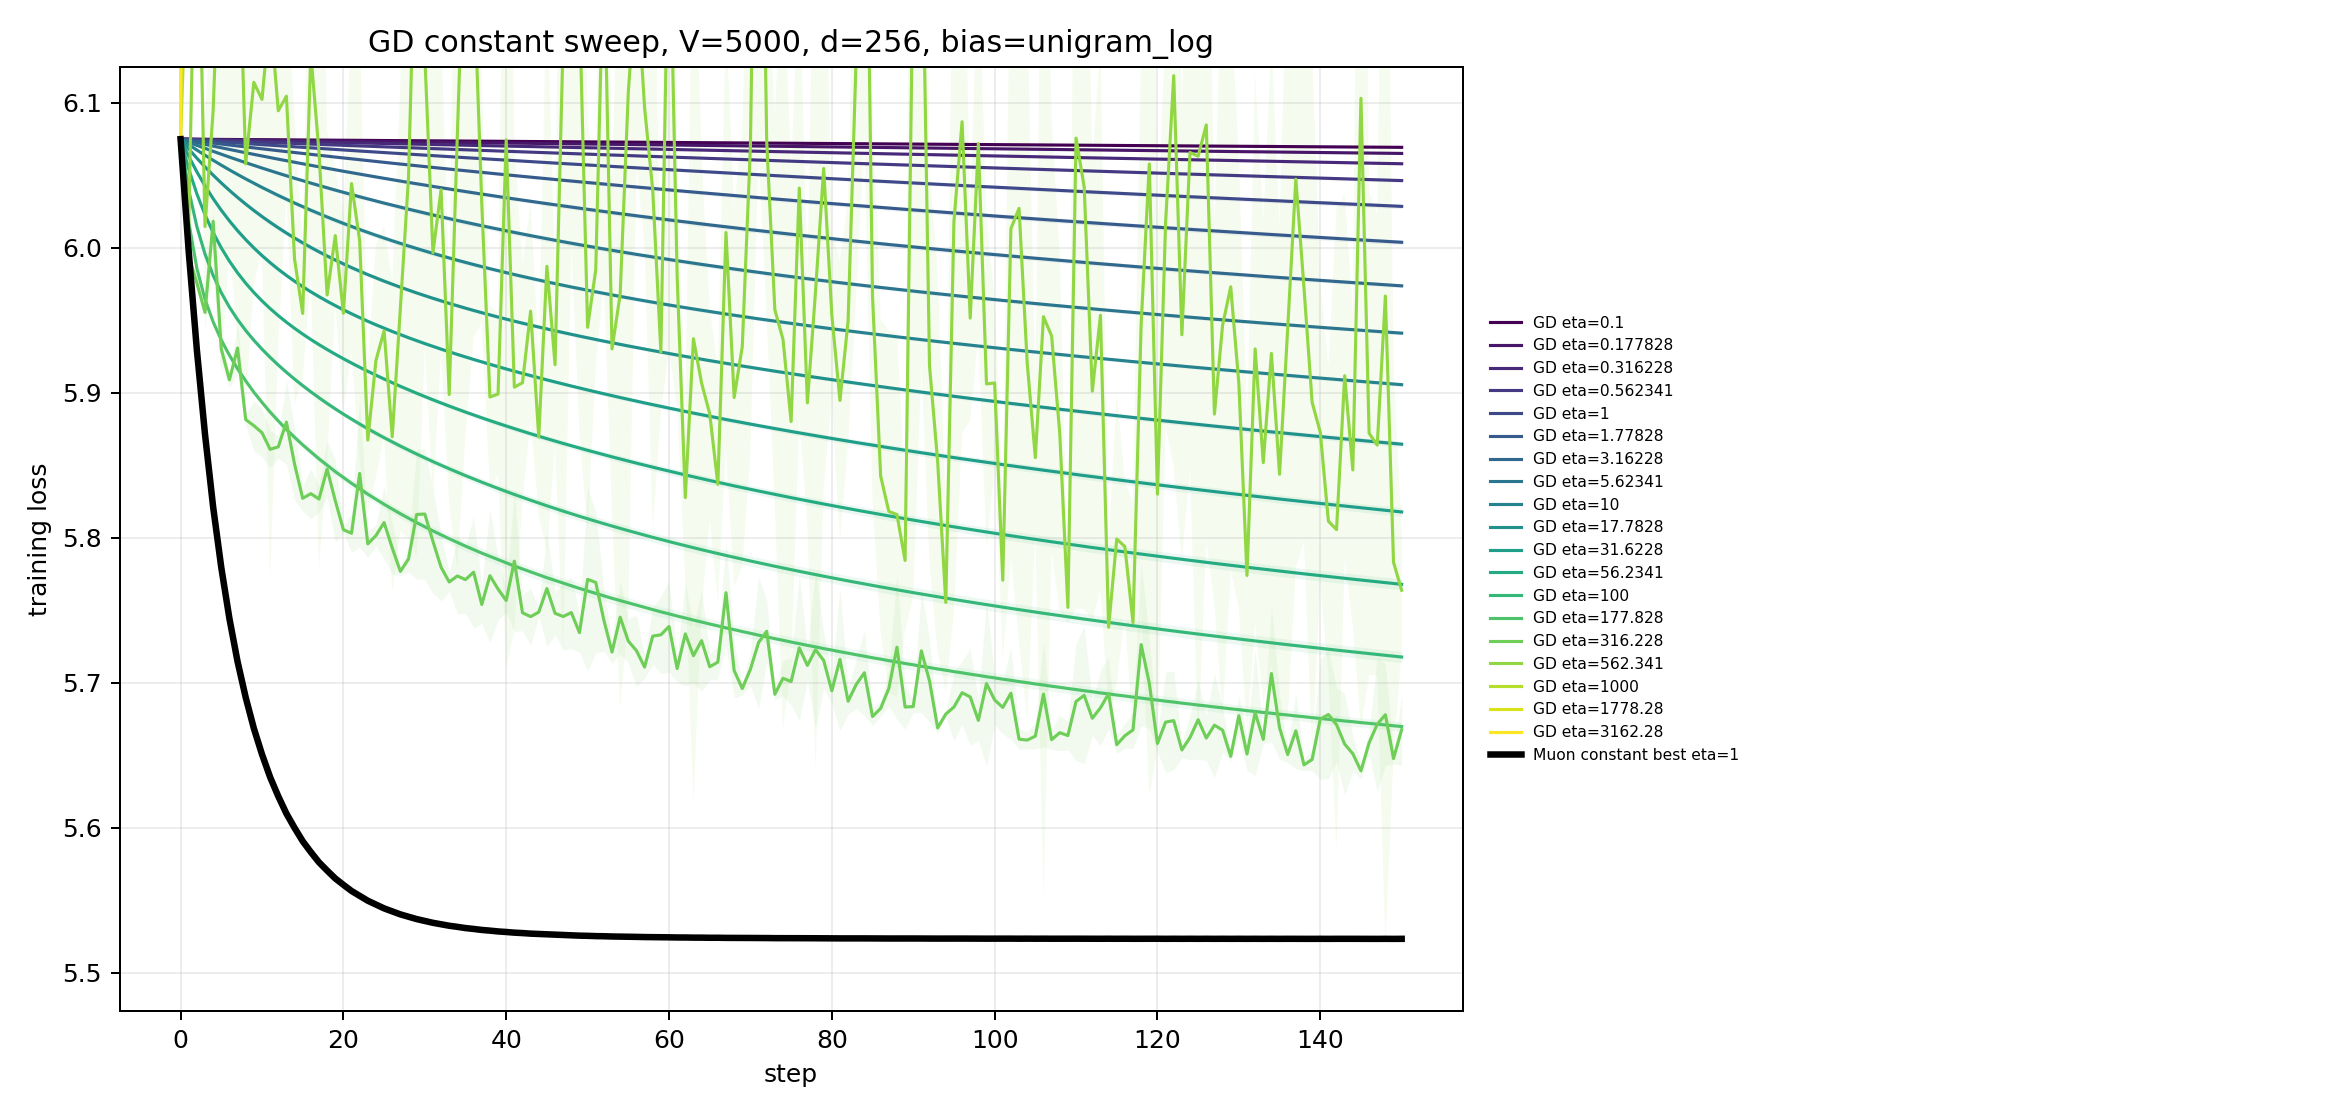
\includegraphics[width=\linewidth]{figures/report_figures/gd_constant_sweep_V5000_d256_rho1e-03_unigram_log.png}
\caption{GD sweep.}
\end{subfigure}\hfill
\begin{subfigure}[t]{0.9\linewidth}
\centering
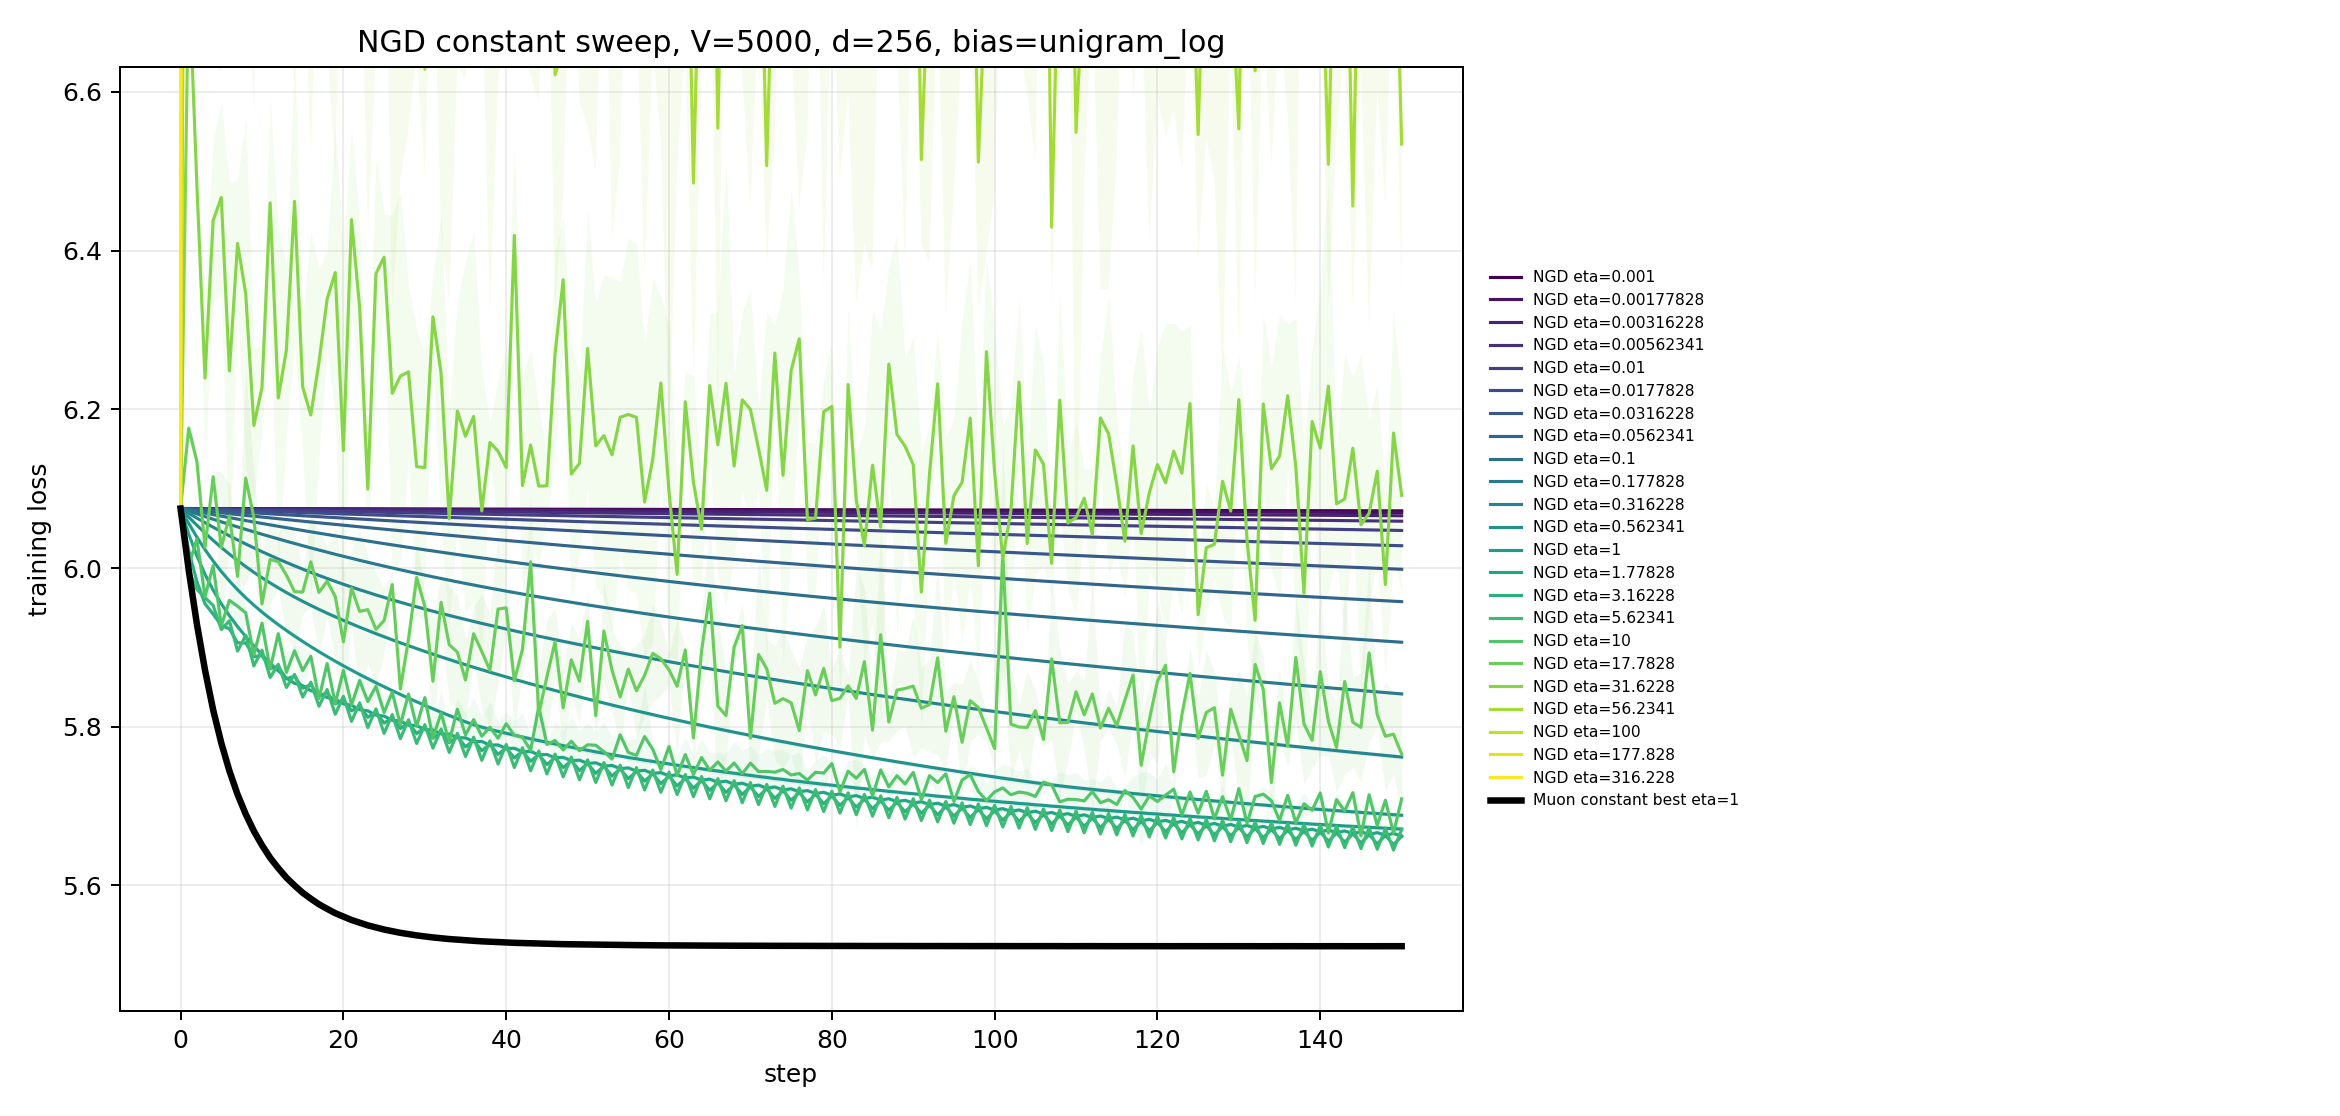
\includegraphics[width=\linewidth]{figures/report_figures/ngd_constant_sweep_V5000_d256_rho1e-03_unigram_log.png}
\caption{NGD sweep.}
\end{subfigure}
\caption{\textbf{\(V=5000\), \(d=256\), \(\rho=10^{-3}\), \texttt{unigram\_log} bias.}
Left: GD constant-\(\eta\) sweep loss curves. Right: NGD constant-\(\eta\) sweep loss curves. Each colored curve is one fixed GD/NGD \(\eta\); the black curve is the AUC-selected Muon constant baseline. Curves are seed means with one-standard-deviation bands.}
\label{fig:sweep-unigram-d256}
\end{figure}

\begin{figure}[H]
\centering
\begin{subfigure}[t]{0.9\linewidth}
\centering
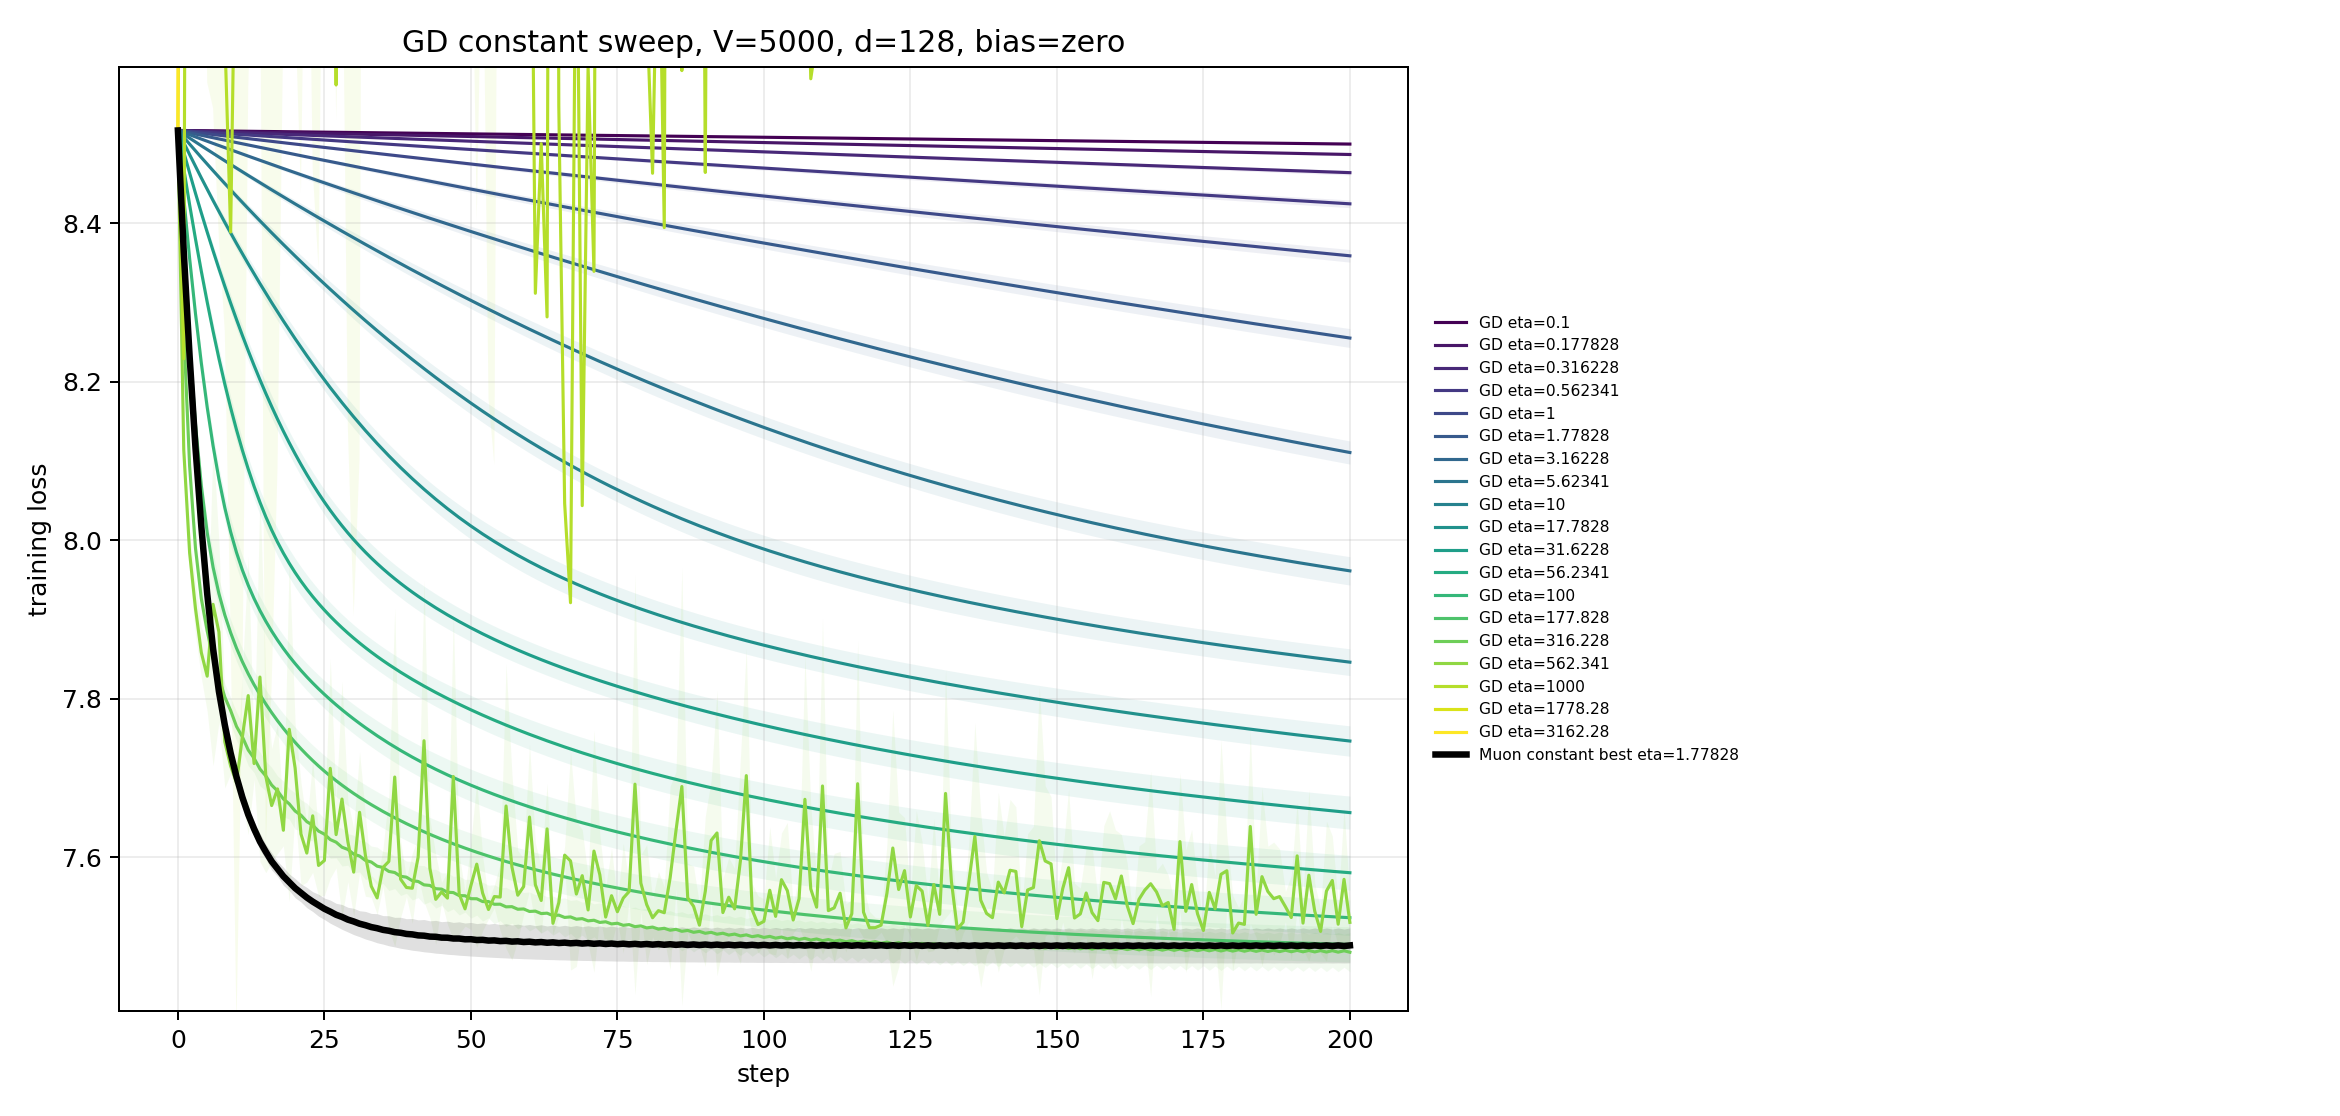
\includegraphics[width=\linewidth]{figures/report_figures/gd_constant_sweep_V5000_d128_rho1e-03_zero.png}
\caption{GD sweep.}
\end{subfigure}\hfill
\begin{subfigure}[t]{0.9\linewidth}
\centering
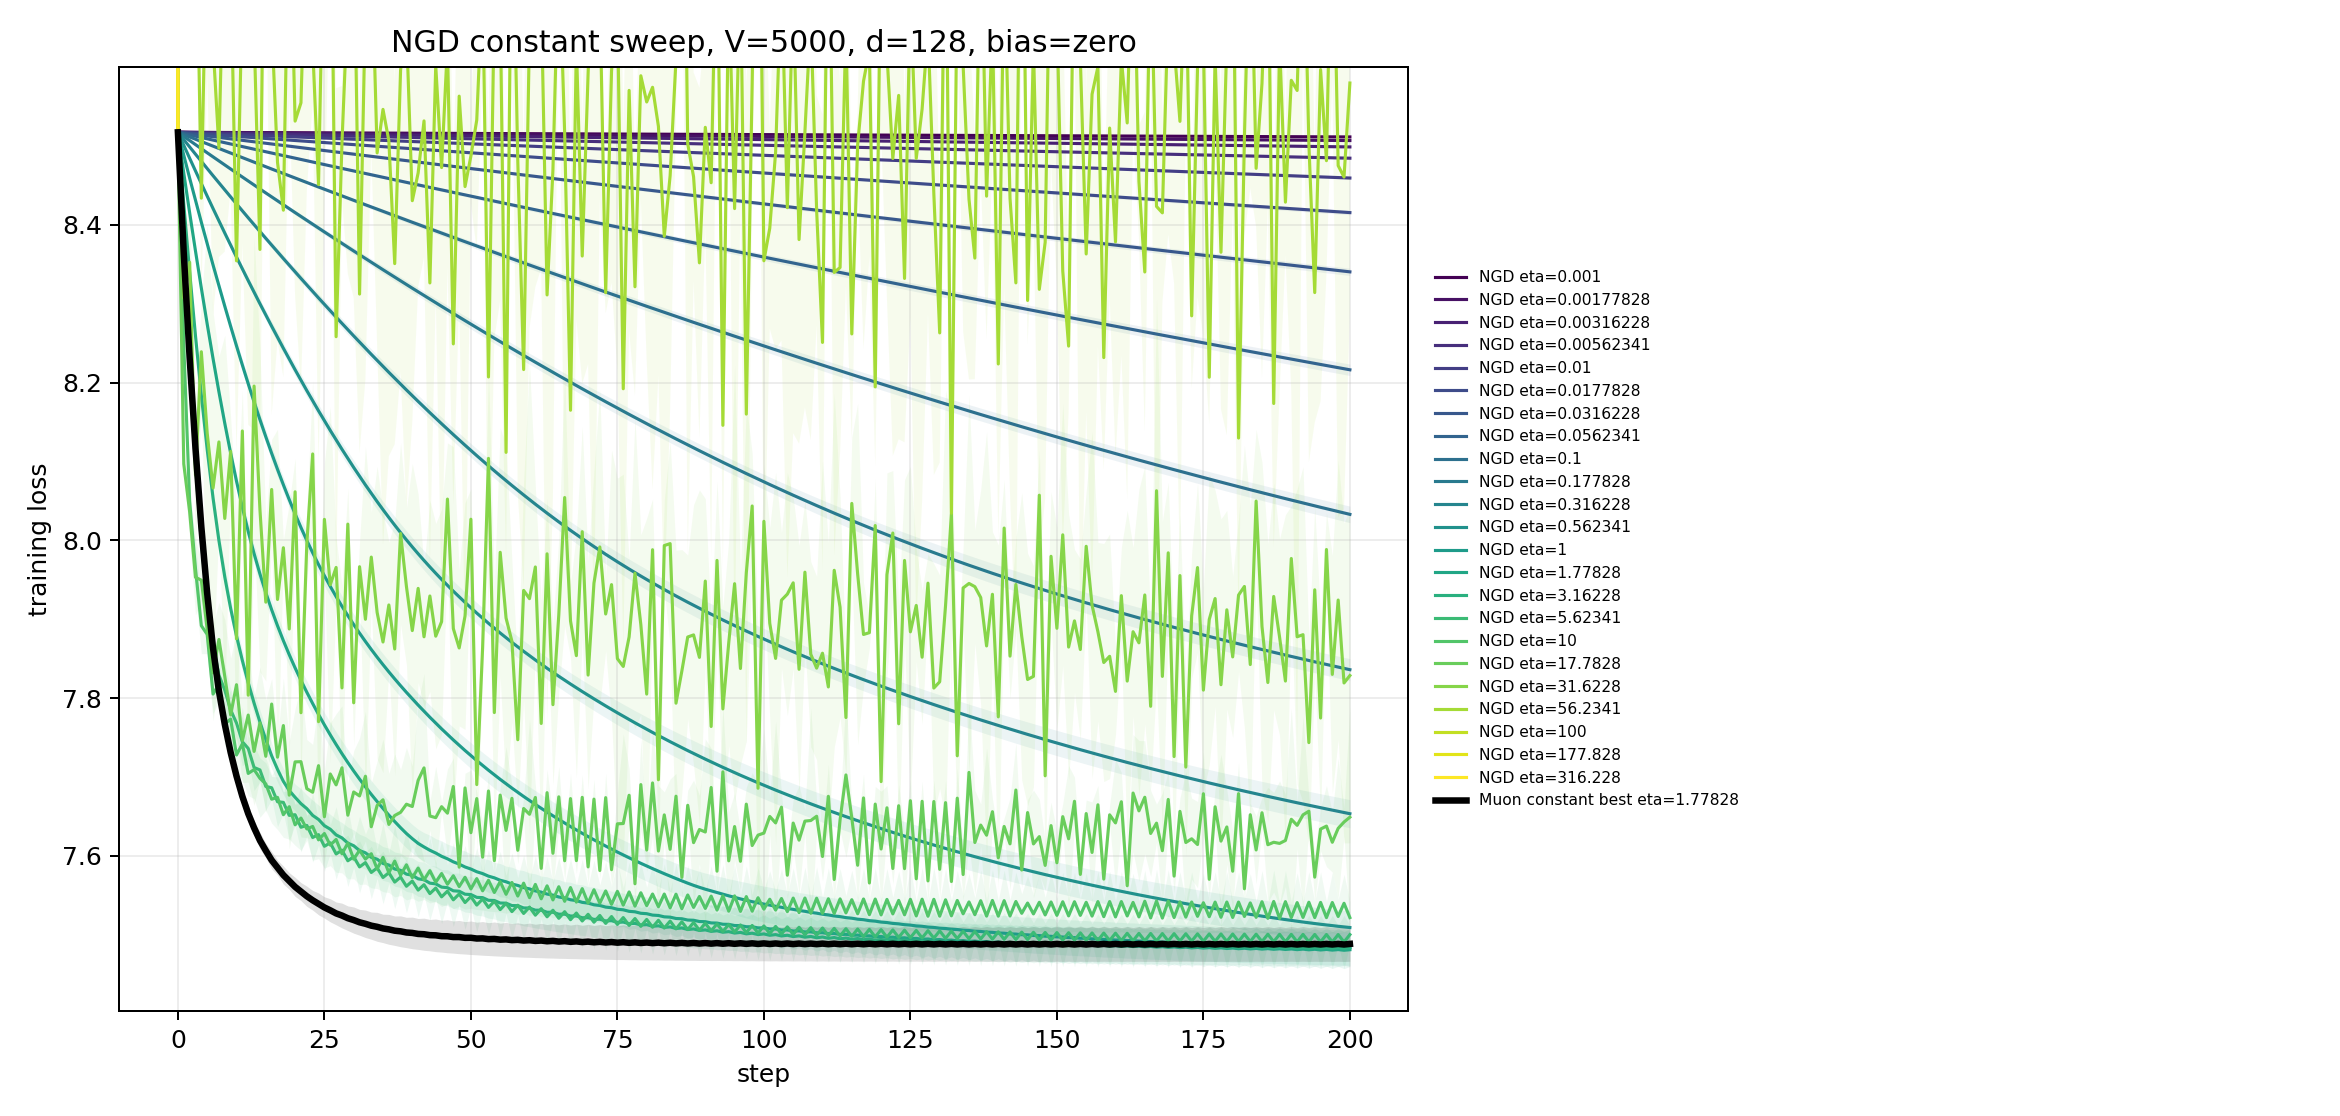
\includegraphics[width=\linewidth]{figures/report_figures/ngd_constant_sweep_V5000_d128_rho1e-03_zero.png}
\caption{NGD sweep.}
\end{subfigure}
\caption{\textbf{\(V=5000\), \(d=128\), \(\rho=10^{-3}\), zero bias.}
Left: GD constant-\(\eta\) sweep loss curves. Right: NGD constant-\(\eta\) sweep loss curves. Each colored curve is one fixed GD/NGD \(\eta\); the black curve is the AUC-selected Muon constant baseline. Curves are seed means with one-standard-deviation bands.}
\label{fig:sweep-zero-d128}
\end{figure}

\begin{figure}[H]
\centering
\begin{subfigure}[t]{0.9\linewidth}
\centering
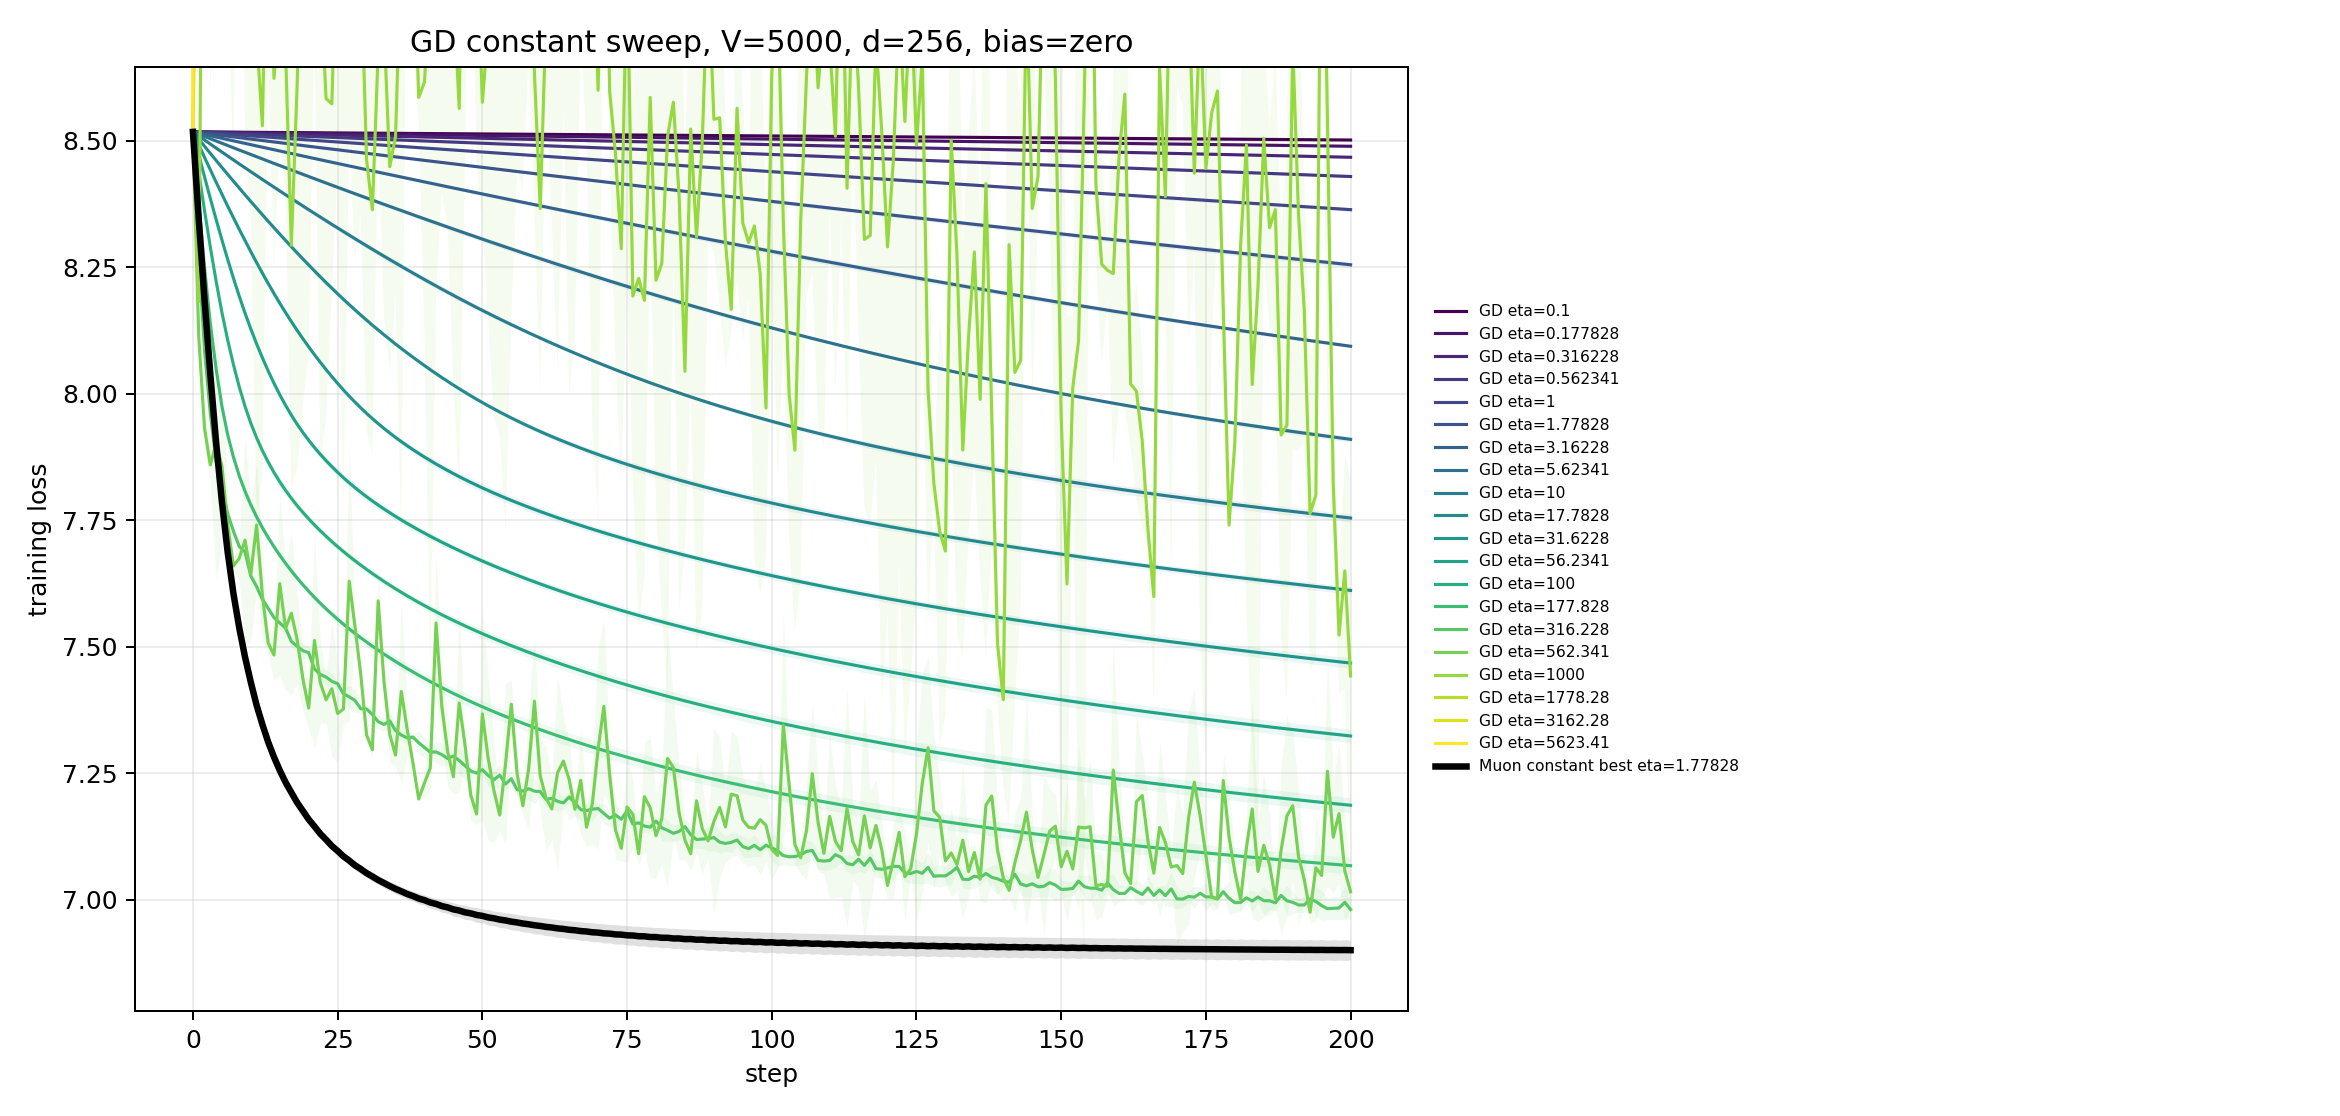
\includegraphics[width=\linewidth]{figures/report_figures/gd_constant_sweep_V5000_d256_rho1e-03_zero.png}
\caption{GD sweep.}
\end{subfigure}\hfill
\begin{subfigure}[t]{0.9\linewidth}
\centering
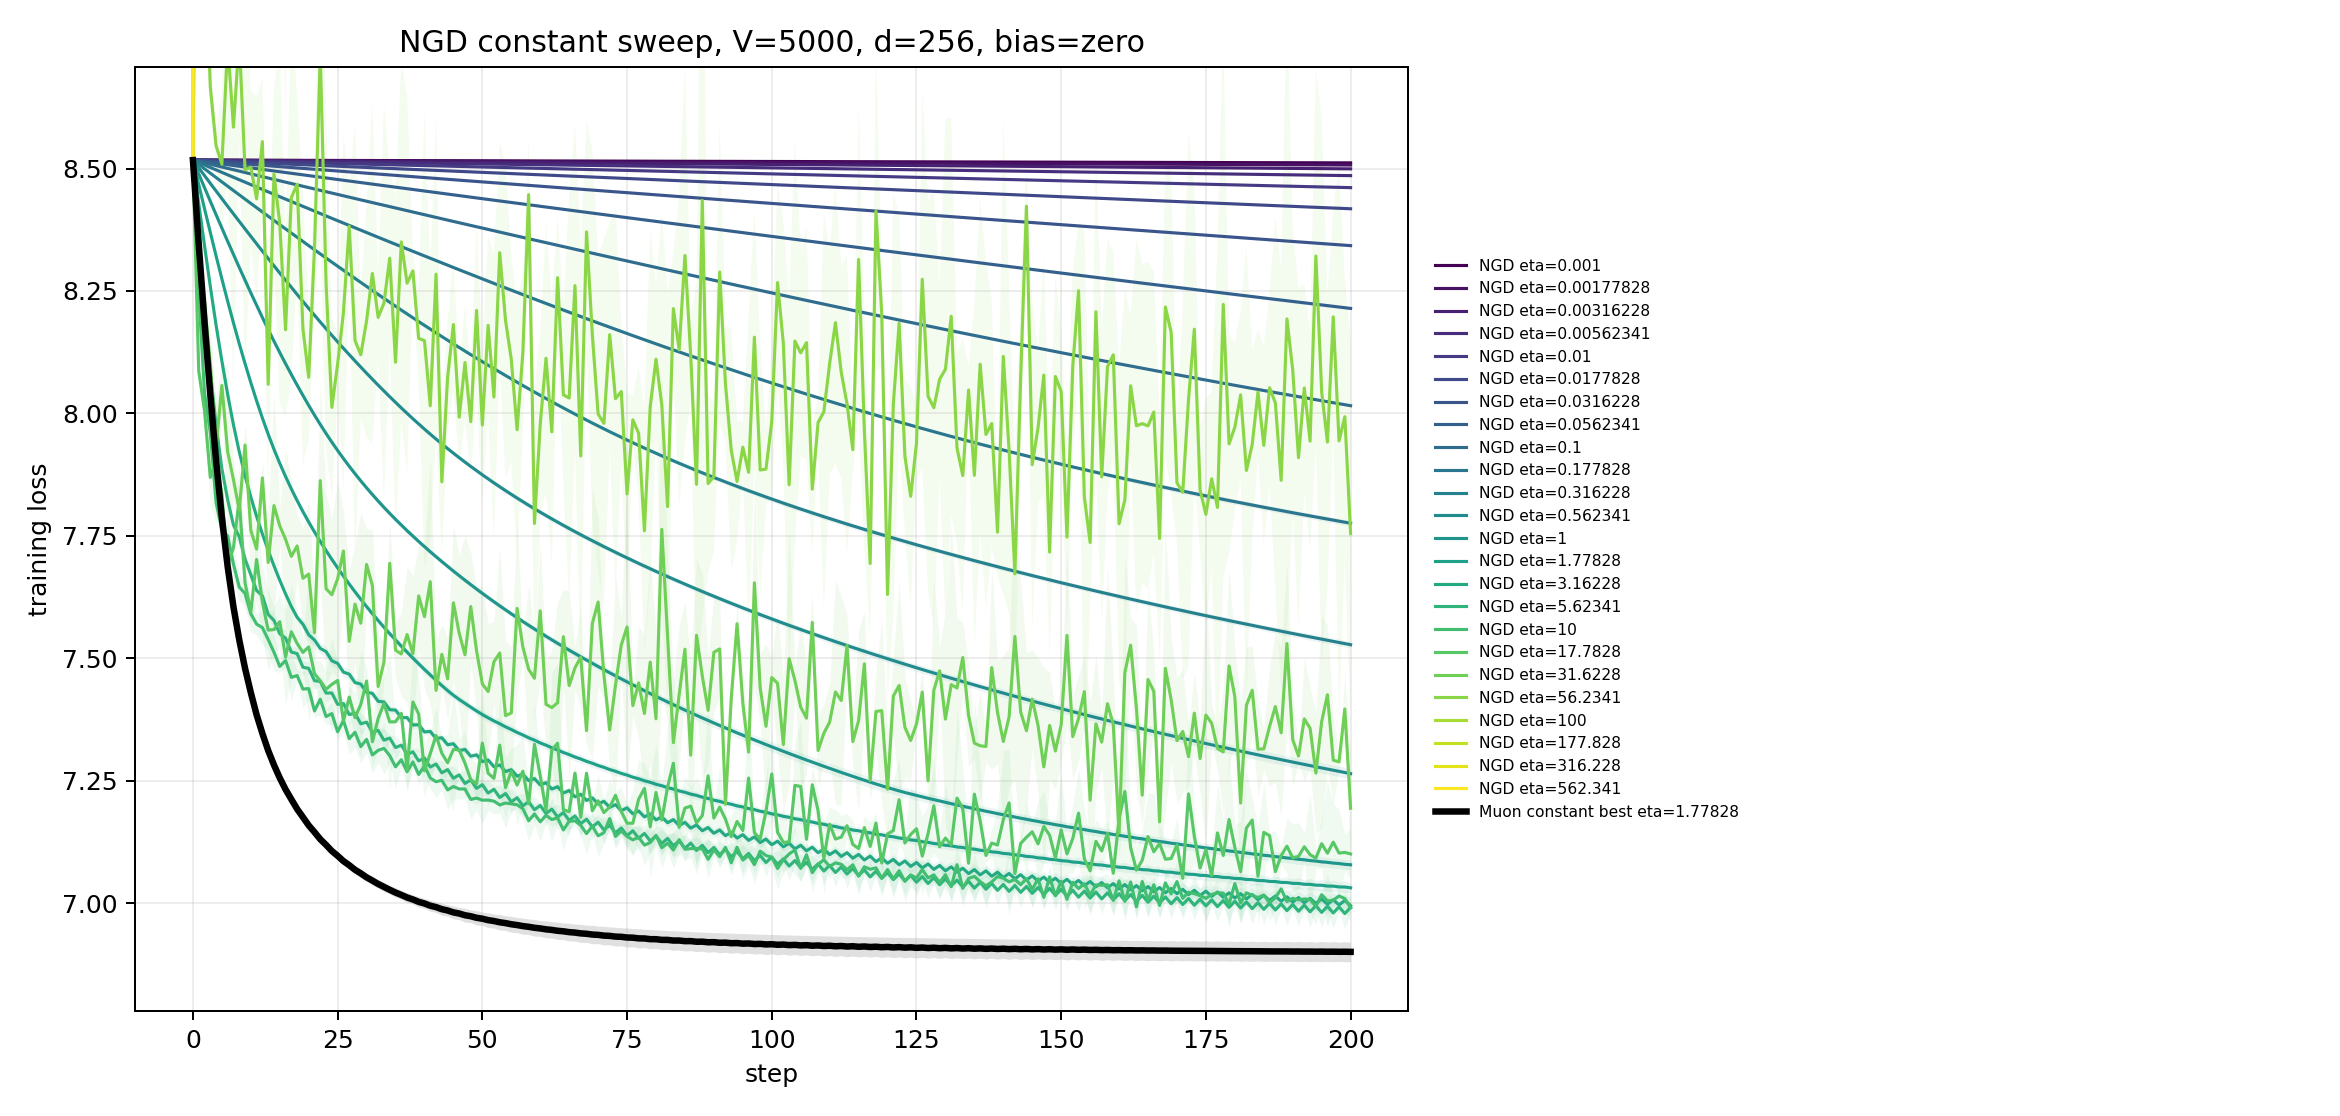
\includegraphics[width=\linewidth]{figures/report_figures/ngd_constant_sweep_V5000_d256_rho1e-03_zero.png}
\caption{NGD sweep.}
\end{subfigure}
\caption{\textbf{\(V=5000\), \(d=256\), \(\rho=10^{-3}\), zero bias.}
Left: GD constant-\(\eta\) sweep loss curves. Right: NGD constant-\(\eta\) sweep loss curves. Each colored curve is one fixed GD/NGD \(\eta\); the black curve is the AUC-selected Muon constant baseline. Curves are seed means with one-standard-deviation bands.}
\label{fig:sweep-zero-d256}
\end{figure}

\FloatBarrier

\section{Data Descriptive Analysis}
\label{sec:data-description}

\paragraph{Notation.}
The empirical bigram count matrix is denoted by \(C\in\mathbb{R}_{\ge 0}^{V\times V}\), where \(C_{y,x}\) counts how often target token \(y\) follows context token \(x\). Let
\begin{equation}
N=\sum_{x=1}^{V}\sum_{y=1}^{V} C_{y,x},
\qquad
P_{y,x}=\frac{C_{y,x}}{N}.
\end{equation}
The context and target marginals are
\begin{equation}
\pi_x=\sum_y P_{y,x},
\qquad
p_y=\sum_x P_{y,x},
\end{equation}
and the empirical conditional next-token distribution is
\begin{equation}
Q(y\mid x)=\frac{P_{y,x}}{\pi_x}
\quad \text{for } \pi_x>0.
\end{equation}
Thus \(P\) is the joint bigram distribution, \(\pi\) is the context frequency distribution, \(p\) is the target frequency distribution, and \(Q(\cdot\mid x)\) is the conditional distribution that the linear bigram model is trying to approximate.

Several descriptive statistics are used below. Marginal entropy and effective vocabulary size are
\begin{equation}
H(p)=-\sum_y p_y\log p_y,
\qquad
V_{\mathrm{eff}}=\exp(H(p)).
\end{equation}
Pointwise mutual information compares an observed bigram to the independent unigram model:
\begin{equation}
\mathrm{PMI}(y,x)=\log\frac{P_{y,x}}{p_y\pi_x}.
\end{equation}
For each context \(x\), the conditional entropy, top-1 conditional probability, and deviation from the global target marginal are
\begin{align}
H(Y\mid x)&=-\sum_y Q(y\mid x)\log Q(y\mid x),\\
\mathrm{top1}(x)&=\max_y Q(y\mid x),\\
\mathrm{KL}(Q(\cdot\mid x)\Vert p)&=\sum_y Q(y\mid x)\log\frac{Q(y\mid x)}{p_y}.
\end{align}
For matrix structure, I use three \(V\times V\) matrices:
\begin{equation}
A_{\mathrm{joint}}=P,\qquad
A_{\mathrm{res}}=P-p\pi^\top,\qquad
(A_{\mathrm{corr}})_{y,x}=\frac{P_{y,x}-p_y\pi_x}{\sqrt{p_y\pi_x}}.
\end{equation}
If \(s_1\ge s_2\ge\cdots\) are singular values of a matrix \(A\), the top-\(k\) Frobenius energy is
\begin{equation}
E_k(A)=\frac{\sum_{i=1}^{k}s_i^2}{\sum_i s_i^2}.
\end{equation}

\paragraph{Descriptive setup.}
This section analyzes only the \(V=5000\) PTB train bigram dataset used in the schedule experiments. The train split contains \(N=929{,}588\) bigram observations and 206,760 observed bigram types, so the observed density in the \(5000^2\) bigram matrix is \(0.827\%\). Tokens and contexts are ordered by decreasing marginal frequency when rank-based plots or matrices are shown. Matrix heatmaps display \(\log_{10}(Q(y\mid x)+10^{-6})\), which makes sparse low-probability structure visible without changing the underlying column-normalized conditionals.

\begin{table}[t]
\centering
\begin{tabular}{lr}
\toprule
Quantity & Value \\
\midrule
Vocabulary size \(V\) & 5000 \\
Train bigrams \(N\) & 929,588 \\
Observed bigram types & 206,760 \\
Observed bigram density & 0.827\% \\
Target entropy \(H(p)\) & 6.075 nats \\
Effective vocabulary \(\exp(H(p))\) & 434.87 \\
Weighted conditional entropy \(H(Y\mid X)\) & 4.143 nats \\
Mutual information \(I(X;Y)\) & 1.932 nats \\
Weighted top-1 conditional probability & 0.211 \\
\bottomrule
\end{tabular}
\caption{\textbf{Basic \(V=5000\) train-set statistics.}
All quantities are computed from the empirical PTB bigram distribution \(P_{y,x}\).}
\label{tab:data-basic-stats}
\end{table}

\paragraph{Marginal concentration.}
Figure~\ref{fig:data-marginals-v5000} shows that the context and target marginals are nearly identical after sorting by frequency. This is expected for adjacent-token bigrams in a long corpus: except for sentence-boundary effects, the distribution of words appearing as contexts and as next-token targets is almost the same. The marginal rank-frequency curve is strongly Zipf-like. Fitting the target marginal over ranks 10--1000 gives
\[
p_{(i)}\approx c\,i^{-\alpha},
\qquad
\alpha=0.941.
\]
The cumulative mass curve shows why this matters for the optimization objective. Although \(V=5000\), the effective vocabulary is only \(\exp(H(p))=434.87\). The top 10 tokens carry 35.2\% of target mass, the top 100 carry 59.0\%, and the top 1000 carry 83.8\%. Since the loss is a \(\pi_x\)-weighted average over contexts, high-frequency contexts dominate the raw objective and gradient signal.

\begin{figure}[H]
\centering
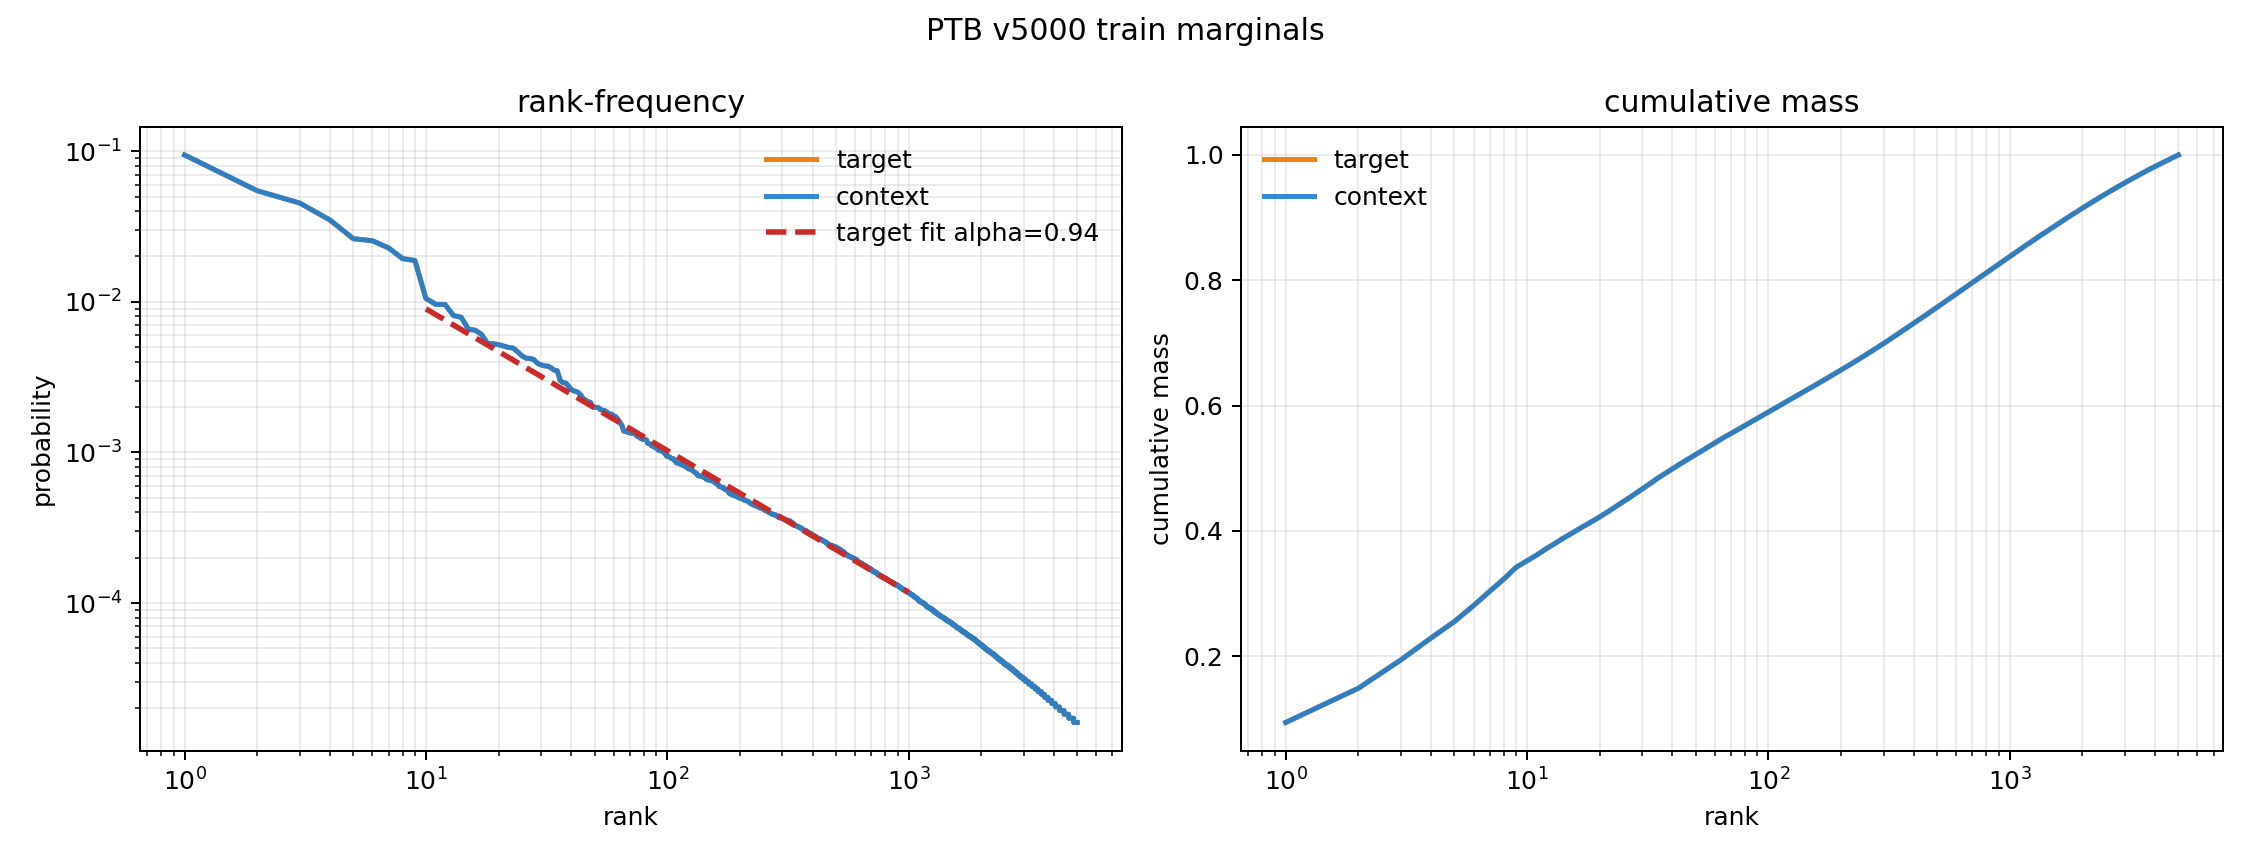
\includegraphics[width=0.95\linewidth]{figures/report_figures/ptb_v5000_train_marginals_zipf_cumulative.png}
\caption{\textbf{Marginal rank-frequency and cumulative mass for \(V=5000\) train.}
Left: sorted context and target marginal probabilities, with a target Zipf fit over ranks 10--1000. Right: cumulative mass captured by the top-ranked context/target tokens.}
\label{fig:data-marginals-v5000}
\end{figure}

\paragraph{Observed bigrams and PMI.}
The bigram matrix is sparse even though the marginal distributions are concentrated. Only 206,760 of the \(25\) million possible \((y,x)\) pairs are observed. Among the observed entries, mass is still heavy-tailed: the top 10 observed bigrams carry 7.07\% of total bigram mass, the top 100 carry 18.7\%, and the top 1000 carry 34.9\%. Figure~\ref{fig:data-bigram-pmi-v5000} shows this rank-frequency decay on the left.

The PMI histogram on the right is weighted by \(P_{y,x}\), not by the number of distinct bigram types. If PTB were well described by an independent unigram model \(P_{y,x}=p_y\pi_x\), most probability mass would sit near \(\mathrm{PMI}=0\). Instead, the probability mass is broadly spread, with mean PMI equal to the mutual information \(I(X;Y)=1.932\) nats. About 89.1\% of the observed bigram probability mass has positive PMI. This indicates that the next-token distribution is strongly context-specific, not merely a draw from the global unigram target distribution.

\begin{figure}[H]
\centering
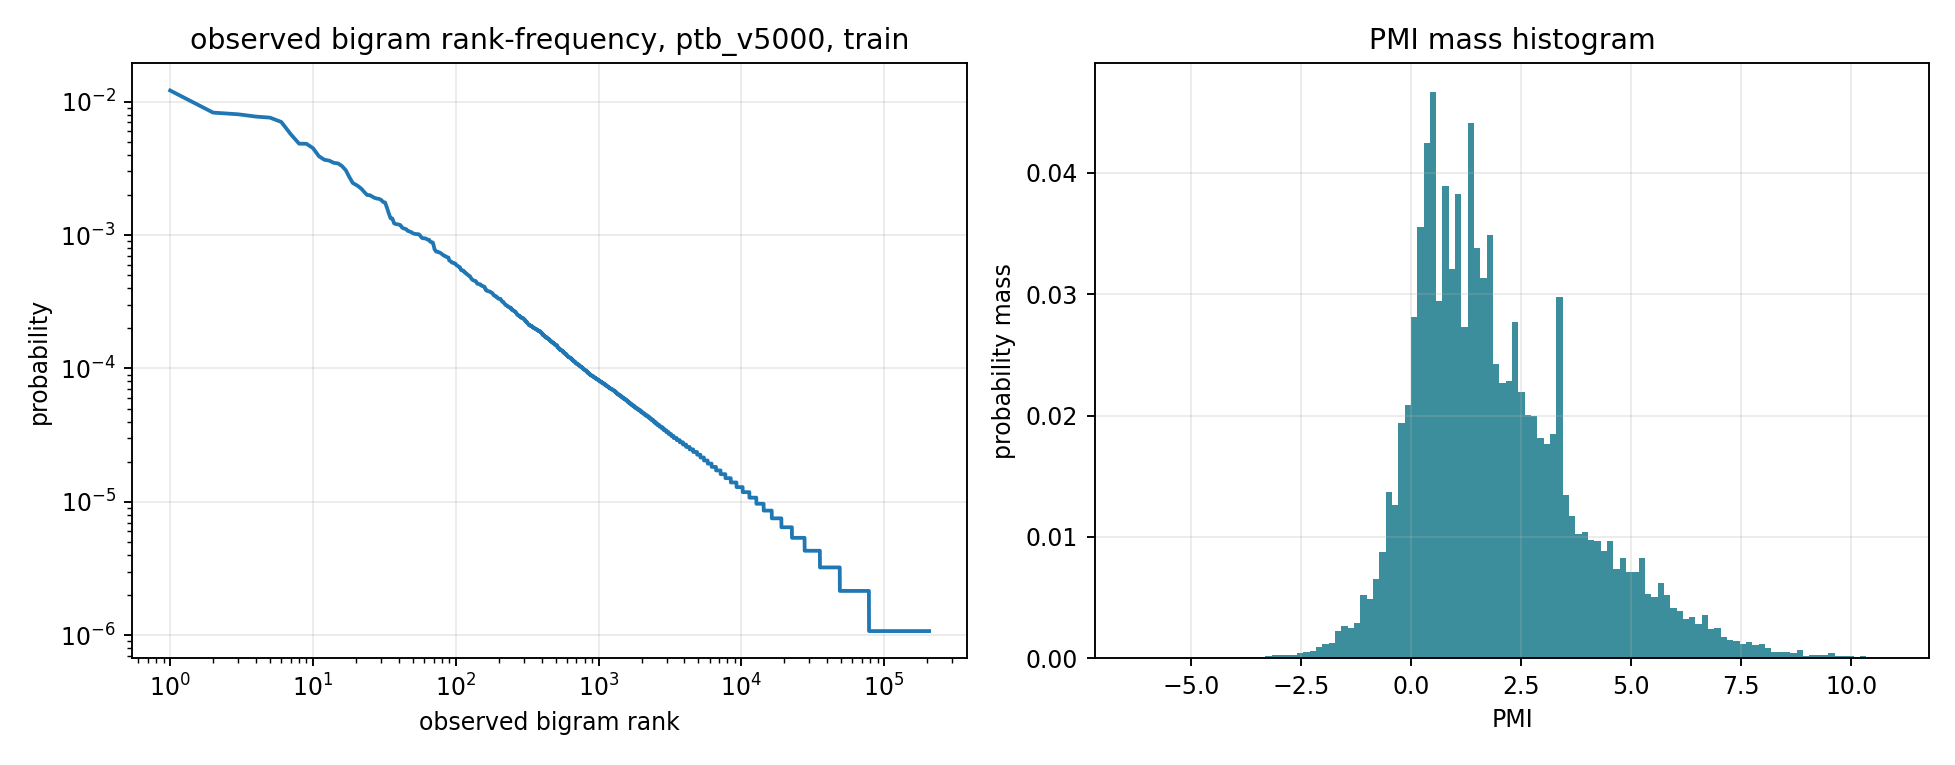
\includegraphics[width=0.95\linewidth]{figures/report_figures/bigram_rank_pmi_ptb_v5000_train.png}
\caption{\textbf{Observed bigram rank-frequency and PMI mass for \(V=5000\) train.}
Left: observed bigram probabilities sorted by rank. Right: probability-mass-weighted histogram of \(\mathrm{PMI}(y,x)\).}
\label{fig:data-bigram-pmi-v5000}
\end{figure}

\paragraph{Context-level conditional structure.}
Figure~\ref{fig:data-context-structure-v5000} plots one point per context token. The x-axis is context count, so the plots separate rare contexts from high-mass contexts. Frequent contexts have many more observed next-token types and higher conditional entropy; the most frequent contexts can have hundreds or thousands of distinct observed targets. Rare contexts often have very small empirical support, which makes their conditional distributions sharp and gives them high top-1 probability.

The KL plot is especially important. It measures how far \(Q(\cdot\mid x)\) is from the global target marginal \(p\). If contexts merely reproduced unigram frequencies, these values would be close to zero. Instead, many contexts have KL values well above 2 nats, and the weighted context-bucket summary increases from 1.676 nats in the most frequent bucket to 3.726 nats in the rarest bucket. The rare buckets have stronger context-specific distributions, but they carry little probability mass: the top 1000 contexts account for 83.8\% of \(\pi\), while the bottom 1000 account for only 1.84\%. This creates a tension in the objective: high-frequency contexts dominate the loss, but low-frequency contexts show sharper and more idiosyncratic conditional structure.

\begin{figure}[H]
\centering
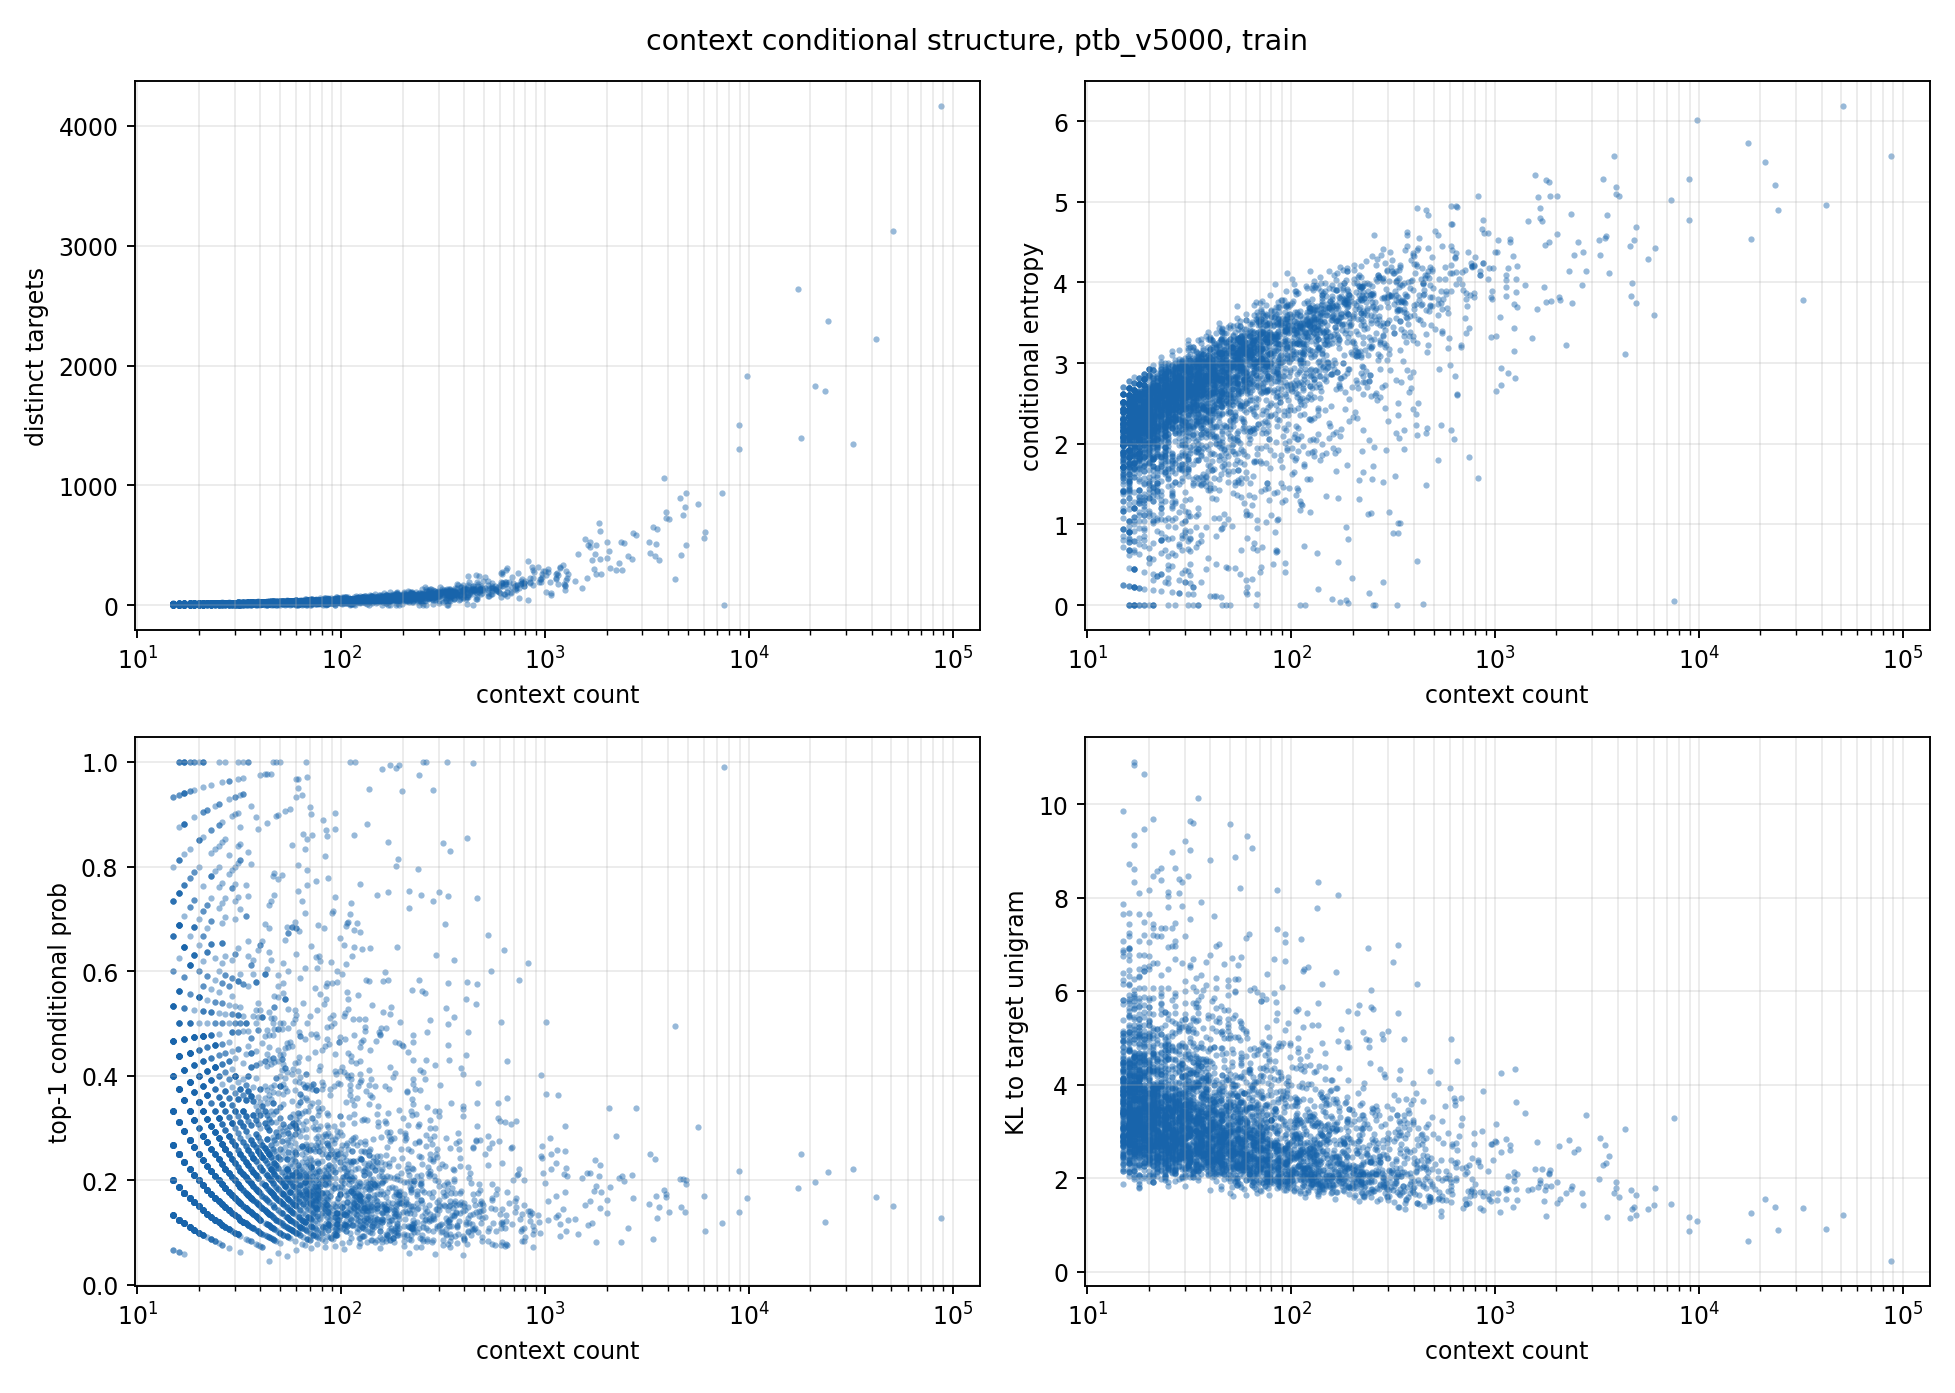
\includegraphics[width=0.95\linewidth]{figures/report_figures/context_structure_ptb_v5000_train.png}
\caption{\textbf{Context conditional structure for \(V=5000\) train.}
Each point is a context token \(x\). The four panels show distinct targets, conditional entropy, top-1 conditional probability, and \(\mathrm{KL}(Q(\cdot\mid x)\Vert p)\) versus context count.}
\label{fig:data-context-structure-v5000}
\end{figure}

\paragraph{Conditional probability matrix.}
The conditional matrix \(Q(y\mid x)\) gives a more direct view of the object being modeled. In Figure~\ref{fig:data-conditional-matrix-v5000}, both axes are ordered by context-frequency rank, and each column is a probability distribution over targets. If the next-token distribution were simply the unigram marginal \(p\), the heatmap would be nearly column-invariant, with horizontal bands determined only by target frequency. Instead, the matrix contains column-dependent bright regions and sparse local structure. This is the visual counterpart of the positive PMI and nonzero KL statistics above.

The top-mass crop keeps the first 2828 ranked tokens, which together carry 95.0\% of the context marginal and 95.0\% of the target marginal. The crop is not renormalized; it is a submatrix of the full conditional \(Q\). Within this top block, the mean conditional mass per context is 0.956 and the median is 0.971, so most next-token probability mass remains inside the high-frequency core vocabulary for most contexts. Figure~\ref{fig:data-prefix-mass-v5000} shows this column-by-column: the top 2000 targets have marginal mass 0.915, but individual contexts can put substantially more or less conditional mass on that prefix.

\begin{figure}[H]
\centering
\begin{subfigure}[t]{0.49\linewidth}
\centering
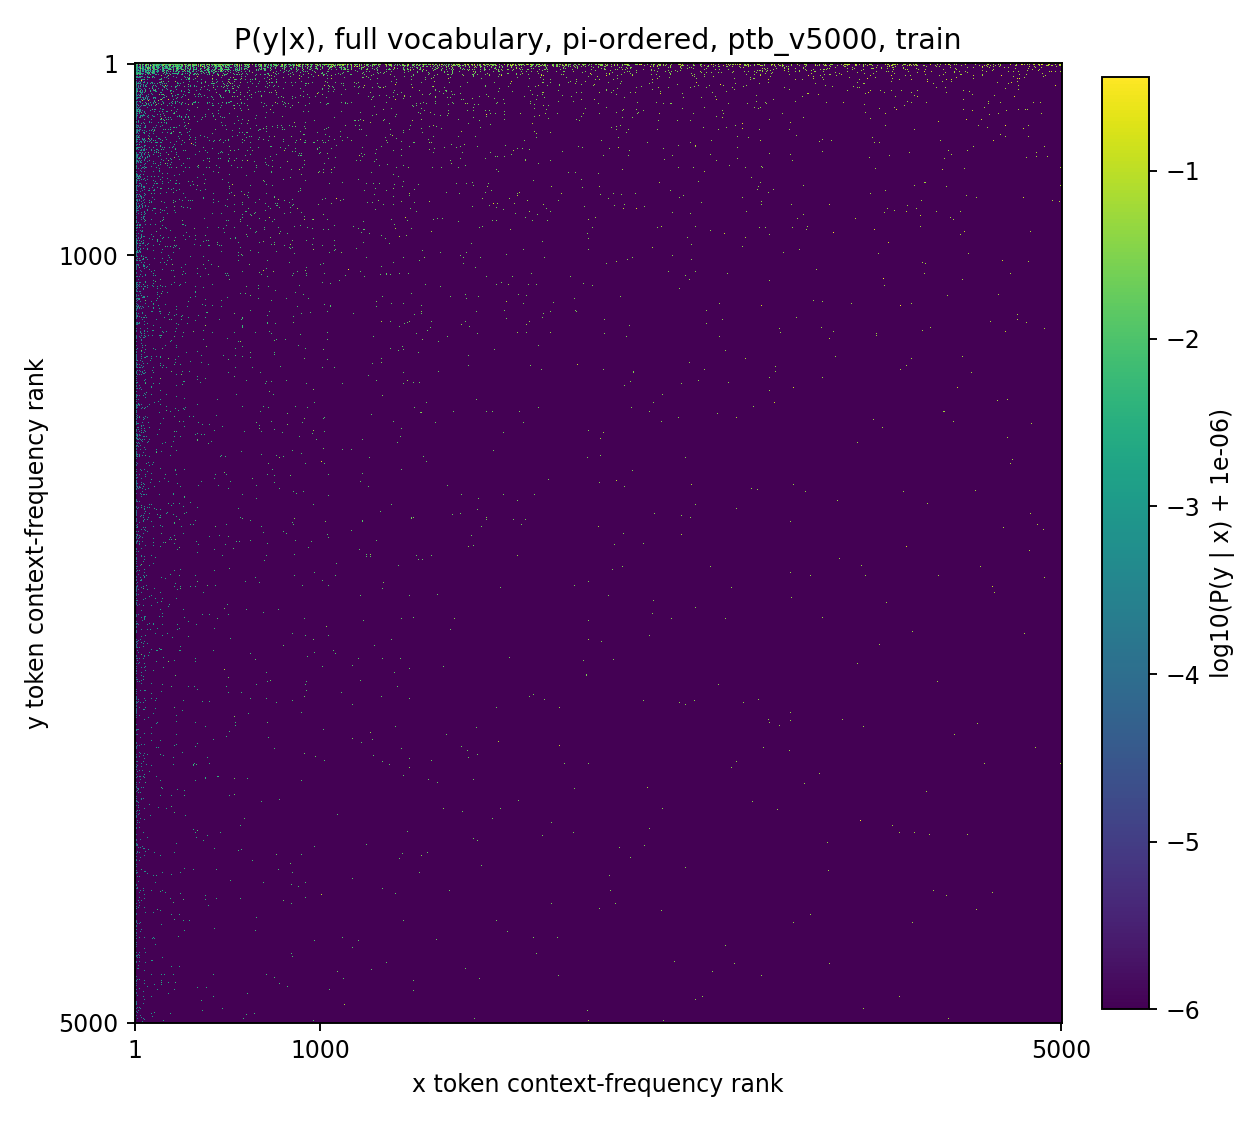
\includegraphics[width=\linewidth]{figures/report_figures/context_ordered_conditional_matrix_ptb_v5000_train.png}
\caption{Full \(5000\times5000\) conditional matrix.}
\end{subfigure}\hfill
\begin{subfigure}[t]{0.49\linewidth}
\centering
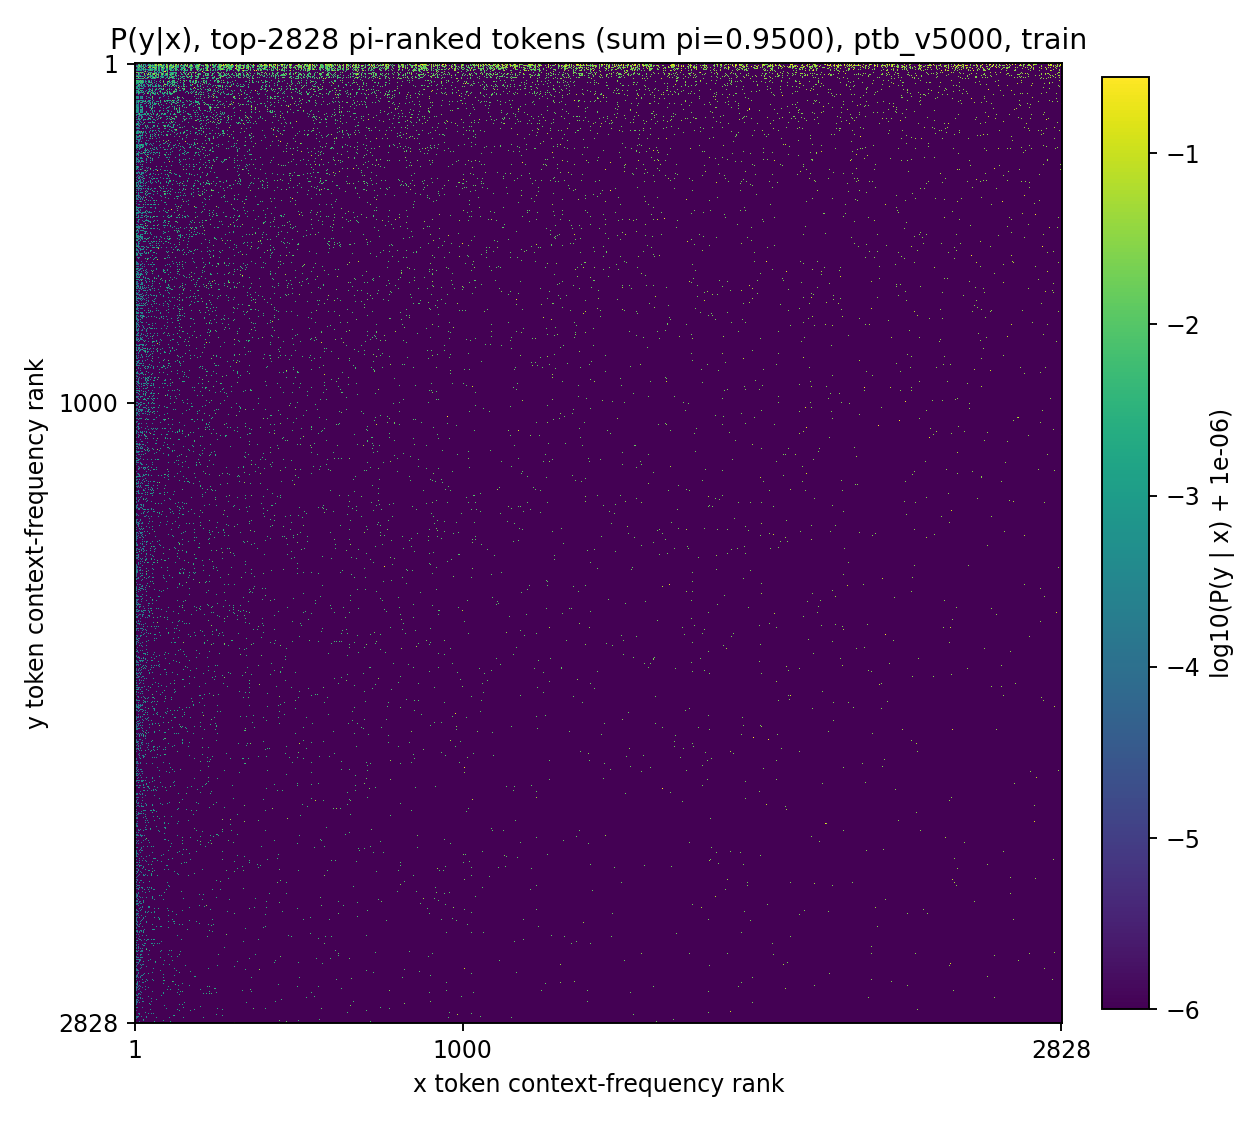
\includegraphics[width=\linewidth]{figures/report_figures/context_ordered_conditional_top2828_mass0.950_ptb_v5000_train.png}
\caption{Top-mass \(2828\times2828\) crop.}
\end{subfigure}
\caption{\textbf{Conditional probability matrix for \(V=5000\) train.}
Entries show \(\log_{10}(Q(y\mid x)+10^{-6})\), with both axes ordered by context-frequency rank.}
\label{fig:data-conditional-matrix-v5000}
\end{figure}

\begin{figure}[H]
\centering
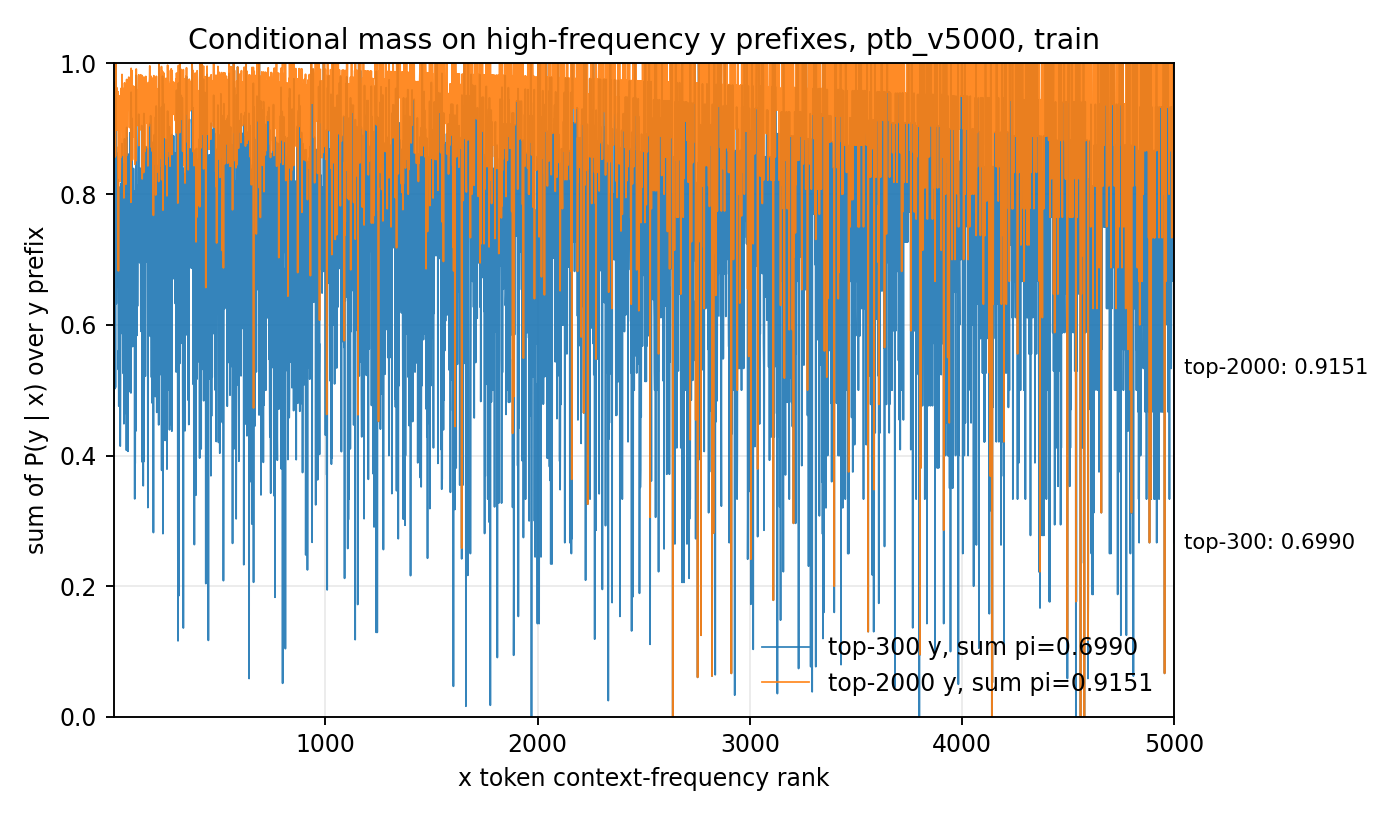
\includegraphics[width=0.78\linewidth]{figures/report_figures/context_ordered_conditional_prefix_mass_curves_ptb_v5000_train.png}
\caption{\textbf{Conditional mass on high-frequency target prefixes.}
For each context \(x\), the plotted quantity is \(M_K(x)=\sum_{\mathrm{rank}(y)\le K}Q(y\mid x)\), shown for \(K=300\) and \(K=2000\).}
\label{fig:data-prefix-mass-v5000}
\end{figure}

\paragraph{Spectral structure of the data matrices.}
Figure~\ref{fig:data-spectrum-v5000} compares the singular spectra of \(P\), the residual \(P-p\pi^\top\), and the standardized correlation matrix. The joint matrix \(P\) is strongly affected by the marginal heavy tail: its top singular direction alone captures 56.1\% of Frobenius energy, and the top 5 capture 94.9\%. More importantly, after subtracting the independent unigram baseline, the residual matrix is still low-rank in probability-mass-weighted terms: the top residual singular direction captures 38.6\%, the top 5 capture 89.5\%, and the top 10 capture 95.0\% of residual Frobenius energy.

This residual spectrum is a data-only signature of strong low-dimensional association structure. It says that the main context-target deviations from independence are not spread evenly across \(V^2\) directions; they are concentrated in a small number of spectral modes. The standardized correlation matrix has a much flatter energy profile because it downweights the raw marginal scale by \(\sqrt{p_y\pi_x}\). Thus the apparent structure depends on whether we view associations by absolute probability mass or by relative deviation from independence. The loss is probability-mass weighted, so the low-rank residual structure is the more directly relevant one for optimization.

\begin{figure}[H]
\centering
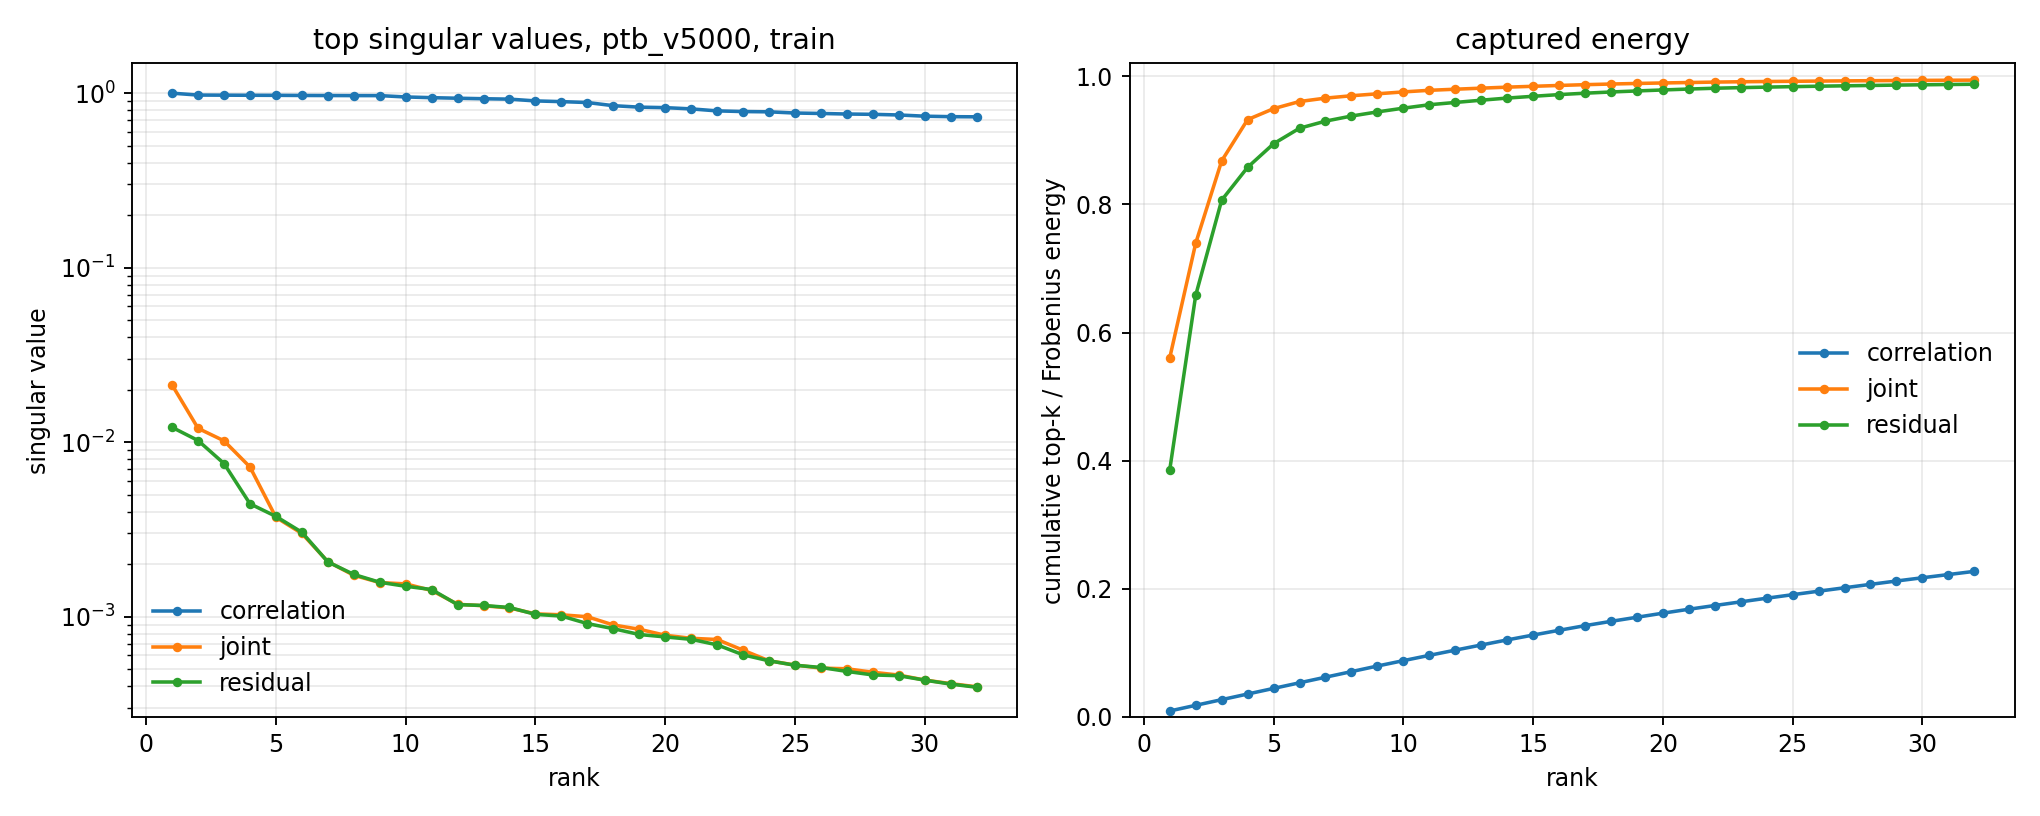
\includegraphics[width=0.95\linewidth]{figures/report_figures/spectrum_ptb_v5000_train.png}
\caption{\textbf{Singular spectra for \(V=5000\) train data matrices.}
Left: top singular values of \(P\), \(P-p\pi^\top\), and the standardized correlation matrix. Right: cumulative Frobenius energy \(E_k\).}
\label{fig:data-spectrum-v5000}
\end{figure}

\paragraph{Optimizer-visible projected gradients.}
The previous spectra are computed directly from the data matrices. The Stage-A optimizer does not update \(P\) directly; it sees the data after projection through the random representations \(U\) and \(E\). At initialization \(W=0\), define the projected target term
\begin{equation}
T=(1-\rho)U^\top P E^\top+\rho\,(U^\top p)(E\pi)^\top,
\qquad \rho=10^{-3}.
\end{equation}
The model term is
\begin{equation}
M=(U^\top q)(E\pi)^\top,
\end{equation}
where \(q=p\) for the \texttt{unigram\_log} bias and \(q_y=1/V\) for the zero bias. The initial projected gradient is then
\begin{equation}
G_0=M-T.
\end{equation}

Figure~\ref{fig:data-projected-gradient-v5000} shows that this projected gradient remains highly spiky after random embedding projection. For \texttt{unigram\_log} bias, the top singular direction carries about 39--40\% of \(G_0\) Frobenius energy, and the top 5 carry about 90\%. For zero bias, the top singular direction is even more dominant, carrying about 57--60\% of the energy, with the top 5 carrying about 95\%. This is the most direct bridge from the data analysis to the optimizer comparison: GD and NGD scale the full gradient but preserve its singular-value imbalance, whereas Muon replaces the active singular values by a flatter polar factor. Therefore, when \(G_t\) is dominated by a few singular modes, Muon can move more evenly across the active subspace than GD-style updates.

\begin{figure}[H]
\centering
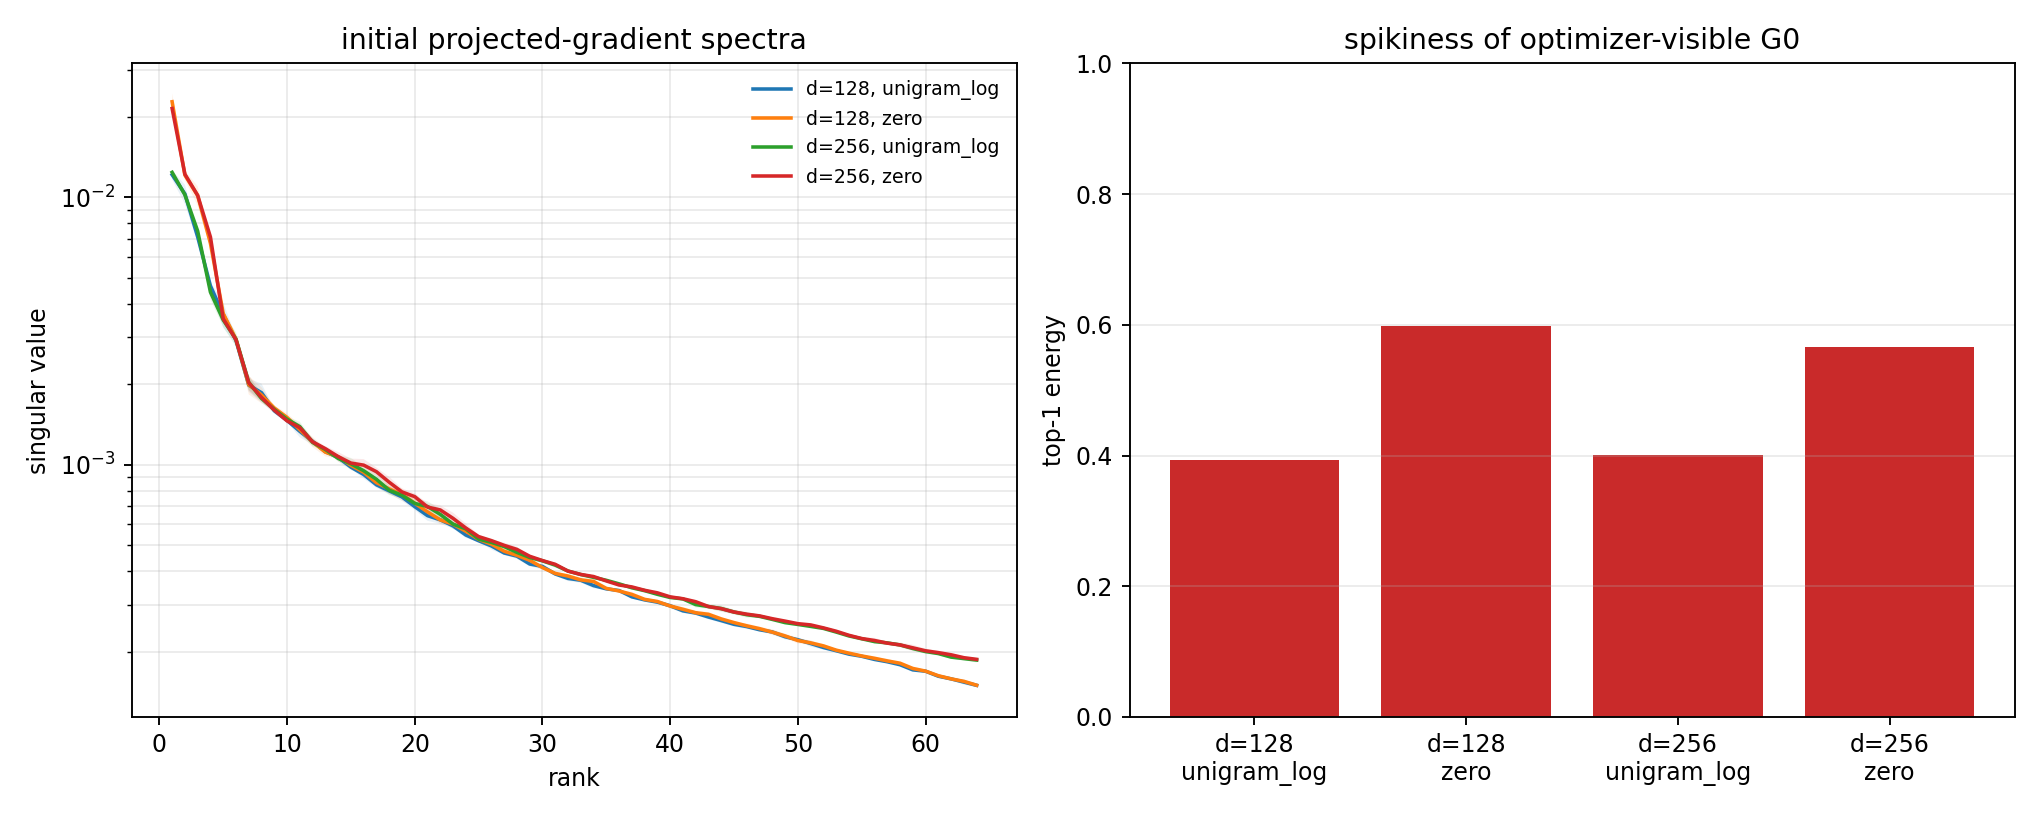
\includegraphics[width=0.95\linewidth]{figures/report_figures/projected_gradient_spectra.png}
\caption{\textbf{Initial projected-gradient spectra for the Stage-A \(V=5000\) setup.}
Left: singular values of \(G_0\) averaged over representation seeds for \(d=128,256\) and both bias choices. Right: top-1 Frobenius energy of \(G_0\).}
\label{fig:data-projected-gradient-v5000}
\end{figure}

\FloatBarrier

\end{document}